\documentclass[12pt,]{article}
\usepackage{lmodern}
\usepackage{amssymb,amsmath}
\usepackage{ifxetex,ifluatex}
\usepackage{fixltx2e} % provides \textsubscript
\ifnum 0\ifxetex 1\fi\ifluatex 1\fi=0 % if pdftex
  \usepackage[T1]{fontenc}
  \usepackage[utf8]{inputenc}
\else % if luatex or xelatex
  \ifxetex
    \usepackage{mathspec}
  \else
    \usepackage{fontspec}
  \fi
  \defaultfontfeatures{Ligatures=TeX,Scale=MatchLowercase}
    \setmainfont[]{Times New Roman}
\fi
% use upquote if available, for straight quotes in verbatim environments
\IfFileExists{upquote.sty}{\usepackage{upquote}}{}
% use microtype if available
\IfFileExists{microtype.sty}{%
\usepackage{microtype}
\UseMicrotypeSet[protrusion]{basicmath} % disable protrusion for tt fonts
}{}
\usepackage[margin=2.54cm]{geometry}
\usepackage{hyperref}
\hypersetup{unicode=true,
            pdftitle={Analysis of US Renewable Energy Electricity Generation Trends},
            pdfauthor={Njeri Kara},
            pdfborder={0 0 0},
            breaklinks=true}
\urlstyle{same}  % don't use monospace font for urls
\usepackage{color}
\usepackage{fancyvrb}
\newcommand{\VerbBar}{|}
\newcommand{\VERB}{\Verb[commandchars=\\\{\}]}
\DefineVerbatimEnvironment{Highlighting}{Verbatim}{commandchars=\\\{\}}
% Add ',fontsize=\small' for more characters per line
\usepackage{framed}
\definecolor{shadecolor}{RGB}{248,248,248}
\newenvironment{Shaded}{\begin{snugshade}}{\end{snugshade}}
\newcommand{\KeywordTok}[1]{\textcolor[rgb]{0.13,0.29,0.53}{\textbf{#1}}}
\newcommand{\DataTypeTok}[1]{\textcolor[rgb]{0.13,0.29,0.53}{#1}}
\newcommand{\DecValTok}[1]{\textcolor[rgb]{0.00,0.00,0.81}{#1}}
\newcommand{\BaseNTok}[1]{\textcolor[rgb]{0.00,0.00,0.81}{#1}}
\newcommand{\FloatTok}[1]{\textcolor[rgb]{0.00,0.00,0.81}{#1}}
\newcommand{\ConstantTok}[1]{\textcolor[rgb]{0.00,0.00,0.00}{#1}}
\newcommand{\CharTok}[1]{\textcolor[rgb]{0.31,0.60,0.02}{#1}}
\newcommand{\SpecialCharTok}[1]{\textcolor[rgb]{0.00,0.00,0.00}{#1}}
\newcommand{\StringTok}[1]{\textcolor[rgb]{0.31,0.60,0.02}{#1}}
\newcommand{\VerbatimStringTok}[1]{\textcolor[rgb]{0.31,0.60,0.02}{#1}}
\newcommand{\SpecialStringTok}[1]{\textcolor[rgb]{0.31,0.60,0.02}{#1}}
\newcommand{\ImportTok}[1]{#1}
\newcommand{\CommentTok}[1]{\textcolor[rgb]{0.56,0.35,0.01}{\textit{#1}}}
\newcommand{\DocumentationTok}[1]{\textcolor[rgb]{0.56,0.35,0.01}{\textbf{\textit{#1}}}}
\newcommand{\AnnotationTok}[1]{\textcolor[rgb]{0.56,0.35,0.01}{\textbf{\textit{#1}}}}
\newcommand{\CommentVarTok}[1]{\textcolor[rgb]{0.56,0.35,0.01}{\textbf{\textit{#1}}}}
\newcommand{\OtherTok}[1]{\textcolor[rgb]{0.56,0.35,0.01}{#1}}
\newcommand{\FunctionTok}[1]{\textcolor[rgb]{0.00,0.00,0.00}{#1}}
\newcommand{\VariableTok}[1]{\textcolor[rgb]{0.00,0.00,0.00}{#1}}
\newcommand{\ControlFlowTok}[1]{\textcolor[rgb]{0.13,0.29,0.53}{\textbf{#1}}}
\newcommand{\OperatorTok}[1]{\textcolor[rgb]{0.81,0.36,0.00}{\textbf{#1}}}
\newcommand{\BuiltInTok}[1]{#1}
\newcommand{\ExtensionTok}[1]{#1}
\newcommand{\PreprocessorTok}[1]{\textcolor[rgb]{0.56,0.35,0.01}{\textit{#1}}}
\newcommand{\AttributeTok}[1]{\textcolor[rgb]{0.77,0.63,0.00}{#1}}
\newcommand{\RegionMarkerTok}[1]{#1}
\newcommand{\InformationTok}[1]{\textcolor[rgb]{0.56,0.35,0.01}{\textbf{\textit{#1}}}}
\newcommand{\WarningTok}[1]{\textcolor[rgb]{0.56,0.35,0.01}{\textbf{\textit{#1}}}}
\newcommand{\AlertTok}[1]{\textcolor[rgb]{0.94,0.16,0.16}{#1}}
\newcommand{\ErrorTok}[1]{\textcolor[rgb]{0.64,0.00,0.00}{\textbf{#1}}}
\newcommand{\NormalTok}[1]{#1}
\usepackage{longtable,booktabs}
\usepackage{graphicx,grffile}
\makeatletter
\def\maxwidth{\ifdim\Gin@nat@width>\linewidth\linewidth\else\Gin@nat@width\fi}
\def\maxheight{\ifdim\Gin@nat@height>\textheight\textheight\else\Gin@nat@height\fi}
\makeatother
% Scale images if necessary, so that they will not overflow the page
% margins by default, and it is still possible to overwrite the defaults
% using explicit options in \includegraphics[width, height, ...]{}
\setkeys{Gin}{width=\maxwidth,height=\maxheight,keepaspectratio}
\IfFileExists{parskip.sty}{%
\usepackage{parskip}
}{% else
\setlength{\parindent}{0pt}
\setlength{\parskip}{6pt plus 2pt minus 1pt}
}
\setlength{\emergencystretch}{3em}  % prevent overfull lines
\providecommand{\tightlist}{%
  \setlength{\itemsep}{0pt}\setlength{\parskip}{0pt}}
\setcounter{secnumdepth}{5}
% Redefines (sub)paragraphs to behave more like sections
\ifx\paragraph\undefined\else
\let\oldparagraph\paragraph
\renewcommand{\paragraph}[1]{\oldparagraph{#1}\mbox{}}
\fi
\ifx\subparagraph\undefined\else
\let\oldsubparagraph\subparagraph
\renewcommand{\subparagraph}[1]{\oldsubparagraph{#1}\mbox{}}
\fi

%%% Use protect on footnotes to avoid problems with footnotes in titles
\let\rmarkdownfootnote\footnote%
\def\footnote{\protect\rmarkdownfootnote}

%%% Change title format to be more compact
\usepackage{titling}

% Create subtitle command for use in maketitle
\newcommand{\subtitle}[1]{
  \posttitle{
    \begin{center}\large#1\end{center}
    }
}

\setlength{\droptitle}{-2em}

  \title{Analysis of US Renewable Energy Electricity Generation Trends}
    \pretitle{\vspace{\droptitle}\centering\huge}
  \posttitle{\par}
  \subtitle{\url{https://github.com/Njeri-Kara/ENVIRON872L-EDA_Final-Project}}
  \author{Njeri Kara}
    \preauthor{\centering\large\emph}
  \postauthor{\par}
    \date{}
    \predate{}\postdate{}
  
\usepackage{booktabs}
\usepackage{longtable}
\usepackage{array}
\usepackage{multirow}
\usepackage{wrapfig}
\usepackage{float}
\usepackage{colortbl}
\usepackage{pdflscape}
\usepackage{tabu}
\usepackage{threeparttable}
\usepackage{threeparttablex}
\usepackage[normalem]{ulem}
\usepackage{makecell}
\usepackage{xcolor}

\begin{document}
\maketitle
\begin{abstract}
Electricity generation in the United States is dominated by fossil
fuel-based technologies.Combustion of fossil fuelsis the main cause of
human-driven emission of greenhouse gases (GHGs).Adoption of rebewable
energy for electricity generation provides an opportunity to mitigate
the negative environmental of fossil fuel fuel adoption. The US
electricity generation has more than doubled since 2008. This paper
analysed the trend in national and state level electricity generation
from major renewable energy sources and found that post 2008 marks a
season of significant change in the adoption trend of renewable energy
resurces particularly wind and solar. It also found that policy changes
could have contributed to this change in renewable energy adoption.
\end{abstract}

\newpage

\tableofcontents  \newpage
\listoftables  \newpage
\listoffigures  \newpage

\textless{}Note: set up autoreferencing for figures and tables in your
document\textgreater{}

\section{Research Question and
Rationale}\label{research-question-and-rationale}

\begin{quote}
Electricity generation in the United States is dominated by fossil
fuel-based technologies. According to the U.S. Energy Information
Administration, In 2018 63.5 \% (EIA, 2018) of the electricity generated
in the country was from fossil fuel based sources such as coal and
natural gas. The combustion of fossil fuels, necessary for electricity
generation, is the main cause of human-driven emission of greenhouse
gases (GHGs) (Quadrelli \& Peterson, 2007) particularly carbon dioxide.
The alternative use of renewable energy provides an opportunity to
decarbonize the electricity sector and mitigate the negative emission
impacts. In the US there appears to be a significant shift in
electricity generation from fossil fuels to renewable energy in the last
decade. EIA estimates that the adoption of renewable energy to generate
electricity has doubled from 2008 to 2019 to account for about 17\%
(EIA, 2018) of the total electricity generation mix.
\end{quote}

\begin{quote}
This paper will aim to:
\end{quote}

\begin{enumerate}
\def\labelenumi{\arabic{enumi}.}
\item
  Research the trend in national level electricity generation from
  renewable energy sources disaggregated by the main renewable sources
  contributing to the growth in total proportion of renewable energy
  generation.
\item
  Investigate the specific trends in wind energy adoption in Kansas and
  solar energy in California to identify any policy change implications
  on renewable energy adoption.
\end{enumerate}

\begin{quote}
Kansas state was selected for the second component of the analysis
because wind energy contributes the largest proportion of the state's
overall electricity generation (36\% as of 2018) compared to other
states. Kansas was also selected because in 2009 it adopted a mandatory
renewable energy policy known as a Renewable Portfolio Standard (RPS)
mandating that the state should generate 20\% of its electricity from
renewable sources by 2025. In 2015, Kansas repealed this policy and
changing the renewable energy goal from mandatory to voluntary (Barbose,
2018). California was selected because solar energy contributes the
largest proportion of the state's overall electricity generation (14\%
as of 2018) compared to other states. California also adopted an RPS
policy in 2002. However, unlike Kansas, it is much more ambitious, it
mandates that the state will generate 60\% of its electricity from
renewable sources by 2030 (Barbose, 2018). Also, unlike Kansas,
California has made several revisions to its renewable energy policy to
strengthen it including in 2006,2007,2011,2015 and 2018 (Barbose, 2018).
\end{quote}

\begin{quote}
The dataset that shall be used for this analysis is the Energy
Information Administration (EIA) data on Monthly total electric power
generation data by State and energy source from 2001 - 2018 available
\href{https://www.eia.gov/electricity/data/state/generation_monthly.xlsx}{here}
\end{quote}

\newpage

\section{Dataset Information}\label{dataset-information}

\begin{quote}
The dataset used for this analysis was Energy Information Administration
(EIA) data on Monthly total electric power generation in Megawatt Hours
(MWh) by State and energy source from 2001 - 2018 obtained from their
site. The data contained excel sheets with monthly totals of electricity
generation by type of power producer and type of energy source in 51
states in the US including national total from January 2001 to January
2019. The dataset included 14 tyoes of energy sources and 6 types of
energy producers:
\end{quote}

\begin{itemize}
\tightlist
\item
  Combined Heat and Power, Commercial Power
\item
  Combined Heat and Power, Electric Power
\item
  Combined Heat and Power, Industrial Power
\item
  Electric Generators, Electric Utilities
\item
  Electric Generators, Independent Power Producers
\item
  Total Electric Power Industry
\end{itemize}

\begin{quote}
The U.S. Renewable Portfolio Standards 2018 Annual Status Report written
by the Lawrence Berkeley National Laboratory was also used as the
reerence source to obtain information on the years states, particularly
Kansas and California, made major revisions to their RPS policies.
\end{quote}

\begin{table}

\caption{\label{tab:unnamed-chunk-2}Summary table of raw dataset}
\centering
\resizebox{\linewidth}{!}{
\begin{tabular}[t]{l|l|l|l|l|l|l}
\hline
  &      YEAR &     MONTH &     STATE &                                         TYPE.OF.PRODUCER &                    ENERGY.SOURCE & GENERATION..Megawatthours.\\
\hline
 & Min.   :2001 & Min.   : 1.000 & CA     : 12945 & Combined Heat and Power, Commercial Power       : 43658 & Total                     : 61824 & Min.   :  -997855\\
\hline
 & 1st Qu.:2005 & 1st Qu.: 3.000 & MI     : 11882 & Combined Heat and Power, Electric Power         : 40674 & Natural Gas               : 56233 & 1st Qu.:     1814\\
\hline
 & Median :2010 & Median : 6.000 & PA     : 11102 & Combined Heat and Power, Industrial Power       : 65061 & Petroleum                 : 53177 & Median :    24701\\
\hline
 & Mean   :2010 & Mean   : 6.479 & NY     : 10654 & Electric Generators, Electric Utilities         : 77347 & Coal                      : 40588 & Mean   :  1416908\\
\hline
 & 3rd Qu.:2014 & 3rd Qu.: 9.000 & MN     : 10393 & Electric Generators, Independent Power Producers: 73257 & Other Biomass             : 38050 & 3rd Qu.:   285558\\
\hline
 & Max.   :2019 & Max.   :12.000 & NC     : 10314 & Total Electric Power Industry                   :111800 & Hydroelectric Conventional: 32771 & Max.   :421796659\\
\hline
 & NA & NA & (Other):344507 & NA & (Other)                   :129154 & NA\\
\hline
\end{tabular}}
\end{table}

\newpage

\section{Exploratory Data Analysis and
Wrangling}\label{exploratory-data-analysis-and-wrangling}

\subsection{Initial data exploration}\label{initial-data-exploration}

\begin{quote}
Explored the raw data set to determine the general structure of the
dataset and variables within it as shown in the code below. This
exploration also included displaying the first 10 rows as shown in Table
2 and last 10 rows of the dataset as shown in Table 3.
\end{quote}

\begin{Shaded}
\begin{Highlighting}[]
\CommentTok{#Summary code}
\CommentTok{#Structure of the dataset}
\KeywordTok{str}\NormalTok{(EIA.data.2001_}\DecValTok{2019}\NormalTok{)}
\end{Highlighting}
\end{Shaded}

\begin{verbatim}
## 'data.frame':    411797 obs. of  6 variables:
##  $ YEAR                      : int  2001 2001 2001 2001 2001 2001 2001 2001 2001 2001 ...
##  $ MONTH                     : int  1 1 1 1 1 1 1 1 1 1 ...
##  $ STATE                     : Factor w/ 53 levels "AK","AL","AR",..: 1 1 1 1 1 1 1 1 1 1 ...
##  $ TYPE.OF.PRODUCER          : Factor w/ 6 levels "Combined Heat and Power, Commercial Power",..: 6 6 6 6 6 6 4 4 4 4 ...
##  $ ENERGY.SOURCE             : Factor w/ 14 levels "Coal","Geothermal",..: 1 9 4 3 13 12 1 9 4 3 ...
##  $ GENERATION..Megawatthours.: int  46903 71085 367521 104549 87 590145 18410 64883 305277 104549 ...
\end{verbatim}

\begin{Shaded}
\begin{Highlighting}[]
\CommentTok{#Collumn names of the variables}
\KeywordTok{colnames}\NormalTok{(EIA.data.2001_}\DecValTok{2019}\NormalTok{)}
\end{Highlighting}
\end{Shaded}

\begin{verbatim}
## [1] "YEAR"                       "MONTH"                     
## [3] "STATE"                      "TYPE.OF.PRODUCER"          
## [5] "ENERGY.SOURCE"              "GENERATION..Megawatthours."
\end{verbatim}

\begin{Shaded}
\begin{Highlighting}[]
\CommentTok{#First 10 rows of the dataset}
\KeywordTok{kable}\NormalTok{(}\KeywordTok{head}\NormalTok{(EIA.data.2001_}\DecValTok{2019}\NormalTok{, }\DecValTok{10}\NormalTok{), }\DataTypeTok{caption =} \StringTok{"First 10 rows of the raw dataset"}\NormalTok{) }\OperatorTok
\StringTok{  }\KeywordTok{kable_styling}\NormalTok{(}\DataTypeTok{latex_options=}\StringTok{"scale_down"}\NormalTok{)}
\end{Highlighting}
\end{Shaded}

\begin{table}

\caption{\label{tab:unnamed-chunk-3}First 10 rows of the raw dataset}
\centering
\resizebox{\linewidth}{!}{
\begin{tabular}[t]{r|r|l|l|l|r}
\hline
YEAR & MONTH & STATE & TYPE.OF.PRODUCER & ENERGY.SOURCE & GENERATION..Megawatthours.\\
\hline
2001 & 1 & AK & Total Electric Power Industry & Coal & 46903\\
\hline
2001 & 1 & AK & Total Electric Power Industry & Petroleum & 71085\\
\hline
2001 & 1 & AK & Total Electric Power Industry & Natural Gas & 367521\\
\hline
2001 & 1 & AK & Total Electric Power Industry & Hydroelectric Conventional & 104549\\
\hline
2001 & 1 & AK & Total Electric Power Industry & Wind & 87\\
\hline
2001 & 1 & AK & Total Electric Power Industry & Total & 590145\\
\hline
2001 & 1 & AK & Electric Generators, Electric Utilities & Coal & 18410\\
\hline
2001 & 1 & AK & Electric Generators, Electric Utilities & Petroleum & 64883\\
\hline
2001 & 1 & AK & Electric Generators, Electric Utilities & Natural Gas & 305277\\
\hline
2001 & 1 & AK & Electric Generators, Electric Utilities & Hydroelectric Conventional & 104549\\
\hline
\end{tabular}}
\end{table}

\begin{Shaded}
\begin{Highlighting}[]
\CommentTok{#Last 10 rows of the dataset}
\KeywordTok{kable}\NormalTok{(}\KeywordTok{tail}\NormalTok{(EIA.data.2001_}\DecValTok{2019}\NormalTok{, }\DecValTok{10}\NormalTok{), }\DataTypeTok{caption =} \StringTok{"Last 10 rows of the raw dataset"}\NormalTok{) }\OperatorTok
\StringTok{  }\KeywordTok{kable_styling}\NormalTok{(}\DataTypeTok{latex_options=}\StringTok{"scale_down"}\NormalTok{)}
\end{Highlighting}
\end{Shaded}

\begin{table}

\caption{\label{tab:unnamed-chunk-3}Last 10 rows of the raw dataset}
\centering
\resizebox{\linewidth}{!}{
\begin{tabular}[t]{l|r|r|l|l|l|r}
\hline
  & YEAR & MONTH & STATE & TYPE.OF.PRODUCER & ENERGY.SOURCE & GENERATION..Megawatthours.\\
\hline
411788 & 2019 & 1 & WY & Electric Generators, Independent Power Producers & Hydroelectric Conventional & 0\\
\hline
411789 & 2019 & 1 & WY & Electric Generators, Independent Power Producers & Natural Gas & 285\\
\hline
411790 & 2019 & 1 & WY & Electric Generators, Independent Power Producers & Solar Thermal and Photovoltaic & 6850\\
\hline
411791 & 2019 & 1 & WY & Electric Generators, Independent Power Producers & Wind & 212257\\
\hline
411792 & 2019 & 1 & WY & Electric Generators, Electric Utilities & Total & 3750439\\
\hline
411793 & 2019 & 1 & WY & Electric Generators, Electric Utilities & Coal & 3492763\\
\hline
411794 & 2019 & 1 & WY & Electric Generators, Electric Utilities & Hydroelectric Conventional & 81780\\
\hline
411795 & 2019 & 1 & WY & Electric Generators, Electric Utilities & Natural Gas & 15131\\
\hline
411796 & 2019 & 1 & WY & Electric Generators, Electric Utilities & Petroleum & 2651\\
\hline
411797 & 2019 & 1 & WY & Electric Generators, Electric Utilities & Wind & 158114\\
\hline
\end{tabular}}
\end{table}

\begin{quote}
Further exploration of the raw dataset was carried out to determine the
different factor types in the variables `TYPE.OF.PRODUCER' and
`ENERGY.SOURCE' and the number of unique factors in the STATE variable.
\end{quote}

\begin{Shaded}
\begin{Highlighting}[]
\CommentTok{#Showing the different factors in TYPE.OF.PRODUCER variable}
\KeywordTok{kable}\NormalTok{(}\KeywordTok{freq}\NormalTok{(EIA.data.2001_}\DecValTok{2019}\OperatorTok{$}\NormalTok{TYPE.OF.PRODUCER), }
      \DataTypeTok{caption =} \StringTok{"Factor types of Type of Producer Variable"}\NormalTok{) }\OperatorTok
\StringTok{  }\KeywordTok{kable_styling}\NormalTok{(}\DataTypeTok{latex_options=}\StringTok{"scale_down"}\NormalTok{)}
\end{Highlighting}
\end{Shaded}

\begin{table}

\caption{\label{tab:unnamed-chunk-4}Factor types of Type of Producer Variable}
\centering
\resizebox{\linewidth}{!}{
\begin{tabular}[t]{l|r|r|r|r|r}
\hline
  & Freq & \% Valid & \% Valid Cum. & \% Total & \% Total Cum.\\
\hline
Combined Heat and Power, Commercial Power & 43658 & 10.601826 & 10.60183 & 10.601826 & 10.60183\\
\hline
Combined Heat and Power, Electric Power & 40674 & 9.877197 & 20.47902 & 9.877197 & 20.47902\\
\hline
Combined Heat and Power, Industrial Power & 65061 & 15.799290 & 36.27831 & 15.799290 & 36.27831\\
\hline
Electric Generators, Electric Utilities & 77347 & 18.782798 & 55.06111 & 18.782798 & 55.06111\\
\hline
Electric Generators, Independent Power Producers & 73257 & 17.789590 & 72.85070 & 17.789590 & 72.85070\\
\hline
Total Electric Power Industry & 111800 & 27.149299 & 100.00000 & 27.149299 & 100.00000\\
\hline
<NA> & 0 & NA & NA & 0.000000 & 100.00000\\
\hline
Total & 411797 & 100.000000 & 100.00000 & 100.000000 & 100.00000\\
\hline
\end{tabular}}
\end{table}

\begin{Shaded}
\begin{Highlighting}[]
\CommentTok{#Showing the different factors in ENERGY.SOURCE variable}
\KeywordTok{kable}\NormalTok{(}\KeywordTok{freq}\NormalTok{(EIA.data.2001_}\DecValTok{2019}\OperatorTok{$}\NormalTok{ENERGY.SOURCE), }
      \DataTypeTok{caption =} \StringTok{"Factor types of Energy Source Variable"}\NormalTok{) }\OperatorTok
\StringTok{  }\KeywordTok{kable_styling}\NormalTok{(}\DataTypeTok{latex_options=}\StringTok{"scale_down"}\NormalTok{)}
\end{Highlighting}
\end{Shaded}

\begin{table}

\caption{\label{tab:unnamed-chunk-4}Factor types of Energy Source Variable}
\centering
\resizebox{\linewidth}{!}{
\begin{tabular}[t]{l|r|r|r|r|r}
\hline
  & Freq & \% Valid & \% Valid Cum. & \% Total & \% Total Cum.\\
\hline
Coal & 40588 & 9.8563127 & 9.856313 & 9.8563127 & 9.856313\\
\hline
Geothermal & 3369 & 0.8181216 & 10.674434 & 0.8181216 & 10.674434\\
\hline
Hydroelectric Conventional & 32771 & 7.9580473 & 18.632482 & 7.9580473 & 18.632482\\
\hline
Natural Gas & 56233 & 13.6555147 & 32.287996 & 13.6555147 & 32.287996\\
\hline
Nuclear & 14302 & 3.4730705 & 35.761067 & 3.4730705 & 35.761067\\
\hline
Other & 29522 & 7.1690663 & 42.930133 & 7.1690663 & 42.930133\\
\hline
Other Biomass & 38050 & 9.2399896 & 52.170123 & 9.2399896 & 52.170123\\
\hline
Other Gases & 15852 & 3.8494695 & 56.019592 & 3.8494695 & 56.019592\\
\hline
Petroleum & 53177 & 12.9134015 & 68.932994 & 12.9134015 & 68.932994\\
\hline
Pumped Storage & 8499 & 2.0638810 & 70.996875 & 2.0638810 & 70.996875\\
\hline
Solar Thermal and Photovoltaic & 12308 & 2.9888513 & 73.985726 & 2.9888513 & 73.985726\\
\hline
Total & 61824 & 15.0132225 & 88.998948 & 15.0132225 & 88.998948\\
\hline
Wind & 20041 & 4.8667183 & 93.865667 & 4.8667183 & 93.865667\\
\hline
Wood and Wood Derived Fuels & 25261 & 6.1343332 & 100.000000 & 6.1343332 & 100.000000\\
\hline
<NA> & 0 & NA & NA & 0.0000000 & 100.000000\\
\hline
Total & 411797 & 100.0000000 & 100.000000 & 100.0000000 & 100.000000\\
\hline
\end{tabular}}
\end{table}

\begin{Shaded}
\begin{Highlighting}[]
\CommentTok{#Showing the number of unique state types in the STATE variable}
\KeywordTok{unique}\NormalTok{(EIA.data.2001_}\DecValTok{2019}\OperatorTok{$}\NormalTok{STATE)}
\end{Highlighting}
\end{Shaded}

\begin{verbatim}
##  [1] AK       AL       AR       AZ       CA       CO       CT      
##  [8] DC       DE       FL       GA       HI       IA       ID      
## [15] IL       IN       KS       KY       LA       MA       MD      
## [22] ME       MI       MN       MO       MS       MT       NC      
## [29] ND       NE       NH       NJ       NM       NV       NY      
## [36] OH       OK       OR       PA       RI       SC       SD      
## [43] TN       TX       UT       VA       VT       WA       WI      
## [50] WV       WY       US-TOTAL US-Total
## 53 Levels: AK AL AR AZ CA CO CT DC DE FL GA HI IA ID IL IN KS KY LA ... US-Total
\end{verbatim}

\begin{Shaded}
\begin{Highlighting}[]
\KeywordTok{length}\NormalTok{(}\KeywordTok{unique}\NormalTok{(EIA.data.2001_}\DecValTok{2019}\OperatorTok{$}\NormalTok{STATE))}
\end{Highlighting}
\end{Shaded}

\begin{verbatim}
## [1] 53
\end{verbatim}

\begin{quote}
The above data exploration revealed the following factors of interest,
\emph{Total Electric Power Industry} in the variable \textbf{Type of
Producer} and \emph{US-TOTAL} and \emph{US-Total} in the \textbf{State}
variable. Further data exploration was carried out to determine if the
\emph{Total Electric Power Industry} factor represents electricity
generation values for the summation of all other types of producers and
the difference between factor \emph{US-TOTAL} and \emph{US-Total}
relevant to total electricity generation in all states (at the national
level).
\end{quote}

\subsubsection{Initial data wrangling to determine variation on Producer
Types and State
factors}\label{initial-data-wrangling-to-determine-variation-on-producer-types-and-state-factors}

\begin{Shaded}
\begin{Highlighting}[]
\CommentTok{#Creating a dataset of elec generation sum for of all types }
\CommentTok{#of producers and comparing it total electric power industry}

\NormalTok{EIA.data.producers <-}\StringTok{ }\NormalTok{EIA.data.2001_}\DecValTok{2019} \OperatorTok
\StringTok{  }\KeywordTok{summarise}\NormalTok{(}\StringTok{`}\DataTypeTok{First 5 producer types (GWh)}\StringTok{`}\NormalTok{ =}\StringTok{ }\KeywordTok{sum}\NormalTok{(}\KeywordTok{as.numeric}\NormalTok{(}
\NormalTok{    GENERATION..Megawatthours.[TYPE.OF.PRODUCER}\OperatorTok{!=}
\StringTok{                                    "Total Electric Power Industry"}\NormalTok{]))}\OperatorTok{/}\DecValTok{1000}\NormalTok{,}
            \StringTok{`}\DataTypeTok{Total Electric Power Industry (GWh)}\StringTok{`}\NormalTok{ =}\StringTok{ }\KeywordTok{sum}\NormalTok{(}\KeywordTok{as.numeric}\NormalTok{(}
\NormalTok{              GENERATION..Megawatthours.[TYPE.OF.PRODUCER}\OperatorTok{==}
\StringTok{                                    "Total Electric Power Industry"}\NormalTok{]))}\OperatorTok{/}\DecValTok{1000}\NormalTok{)}
\end{Highlighting}
\end{Shaded}

\begin{table}

\caption{\label{tab:unnamed-chunk-6}Total electricity generation by producer types.}
\centering
\begin{tabular}[t]{r|r}
\hline
First 5 producer types (GWh) & Total Electric Power Industry (GWh)\\
\hline
291739158 & 291739158\\
\hline
\end{tabular}
\end{table}

\begin{quote}
The total electricity generation of all producer types except `Total
Electric Power Industry' was equal to that of `Total Electric Power
Industry'
\end{quote}

\begin{Shaded}
\begin{Highlighting}[]
\CommentTok{#Creating datasets with and without Us-Total and US-TOTAL factors}
\NormalTok{EIA.Data.only_states <-}\StringTok{ }\NormalTok{EIA.data.2001_}\DecValTok{2019} \OperatorTok
\StringTok{  }\KeywordTok{filter}\NormalTok{(TYPE.OF.PRODUCER}\OperatorTok{==}\StringTok{"Total Electric Power Industry"}\NormalTok{) }\OperatorTok
\StringTok{  }\KeywordTok{filter}\NormalTok{(ENERGY.SOURCE}\OperatorTok{==}\StringTok{"Total"}\NormalTok{) }\OperatorTok
\StringTok{  }\KeywordTok{filter}\NormalTok{(STATE}\OperatorTok{!=}\StringTok{ "US-TOTAL"} \OperatorTok{&}\StringTok{ }\NormalTok{STATE}\OperatorTok{!=}\StringTok{ "US-Total"}\NormalTok{) }\OperatorTok
\StringTok{  }\KeywordTok{mutate}\NormalTok{(}\DataTypeTok{Date =} \KeywordTok{make_date}\NormalTok{(YEAR,MONTH))}

\NormalTok{EIA.Data.only_states.sum <-}\StringTok{ }\NormalTok{EIA.Data.only_states }\OperatorTok
\StringTok{  }\KeywordTok{summarise}\NormalTok{(}\StringTok{`}\DataTypeTok{Total Elec Gen for States (GWh)}\StringTok{`}\NormalTok{ =}\StringTok{ }\KeywordTok{sum}\NormalTok{(}
    \KeywordTok{as.numeric}\NormalTok{(}
\NormalTok{      GENERATION..Megawatthours.))}\OperatorTok{/}\DecValTok{1000}\NormalTok{)}

\NormalTok{EIA.Data.US <-}\StringTok{ }\NormalTok{EIA.data.2001_}\DecValTok{2019} \OperatorTok
\StringTok{  }\KeywordTok{filter}\NormalTok{(TYPE.OF.PRODUCER}\OperatorTok{==}\StringTok{"Total Electric Power Industry"}\NormalTok{) }\OperatorTok
\StringTok{  }\KeywordTok{filter}\NormalTok{(ENERGY.SOURCE}\OperatorTok{==}\StringTok{"Total"}\NormalTok{) }\OperatorTok
\StringTok{  }\KeywordTok{filter}\NormalTok{(STATE}\OperatorTok{==}\StringTok{ "US-TOTAL"} \OperatorTok{|}\StringTok{ }\NormalTok{STATE}\OperatorTok{==}\StringTok{ "US-Total"}\NormalTok{) }\OperatorTok
\StringTok{  }\KeywordTok{mutate}\NormalTok{(}\DataTypeTok{Date =} \KeywordTok{make_date}\NormalTok{(YEAR,MONTH))}

\NormalTok{EIA.Data.US.sum <-}\StringTok{ }\NormalTok{EIA.Data.US }\OperatorTok
\StringTok{  }\KeywordTok{summarise}\NormalTok{(}\StringTok{`}\DataTypeTok{Total Elec Gen US-TOTAL  (GWh)}\StringTok{`}\NormalTok{ =}\StringTok{ }\KeywordTok{sum}\NormalTok{(}
    \KeywordTok{as.numeric}\NormalTok{(}
\NormalTok{      GENERATION..Megawatthours.[STATE}\OperatorTok{==}\StringTok{"US-TOTAL"}\NormalTok{]))}\OperatorTok{/}\DecValTok{1000}\NormalTok{,}
            \StringTok{`}\DataTypeTok{Total Elec Gen US-Total  (GWh)}\StringTok{`}\NormalTok{ =}\StringTok{ }\KeywordTok{sum}\NormalTok{(}
              \KeywordTok{as.numeric}\NormalTok{(}
\NormalTok{                GENERATION..Megawatthours.[STATE}\OperatorTok{==}\StringTok{"US-Total"}\NormalTok{]))}\OperatorTok{/}\DecValTok{1000}\NormalTok{,}
            \StringTok{`}\DataTypeTok{Total Elec Gen US-Both  (GWh)}\StringTok{`}\NormalTok{ =}\StringTok{ }\KeywordTok{sum}\NormalTok{(}
              \KeywordTok{as.numeric}\NormalTok{(}
\NormalTok{                GENERATION..Megawatthours.))}\OperatorTok{/}\DecValTok{1000}\NormalTok{)}

\CommentTok{#Table comparison of electricity generation summation of both datasets}
\NormalTok{EIA.Data.States.US.sum <-}\StringTok{ }\KeywordTok{cbind}\NormalTok{(EIA.Data.only_states.sum,EIA.Data.US.sum)}
\KeywordTok{kable}\NormalTok{(EIA.Data.States.US.sum, }
      \DataTypeTok{caption =} \StringTok{"Sumation of Total Electricity generation for all STATES and both US factors"}\NormalTok{) }\OperatorTok
\StringTok{  }\KeywordTok{kable_styling}\NormalTok{(}\DataTypeTok{latex_options=}\StringTok{"scale_down"}\NormalTok{)}
\end{Highlighting}
\end{Shaded}

\begin{table}

\caption{\label{tab:unnamed-chunk-7}Sumation of Total Electricity generation for all STATES and both US factors}
\centering
\resizebox{\linewidth}{!}{
\begin{tabular}[t]{r|r|r|r}
\hline
Total Elec Gen for States (GWh) & Total Elec Gen US-TOTAL  (GWh) & Total Elec Gen US-Total  (GWh) & Total Elec Gen US-Both  (GWh)\\
\hline
72934791 & 44021141 & 28913648 & 72934789\\
\hline
\end{tabular}}
\end{table}

\textbf{Plot of variation in electricity generation at the US-TOTAL and
US-Total factor level}

\begin{figure}
\centering
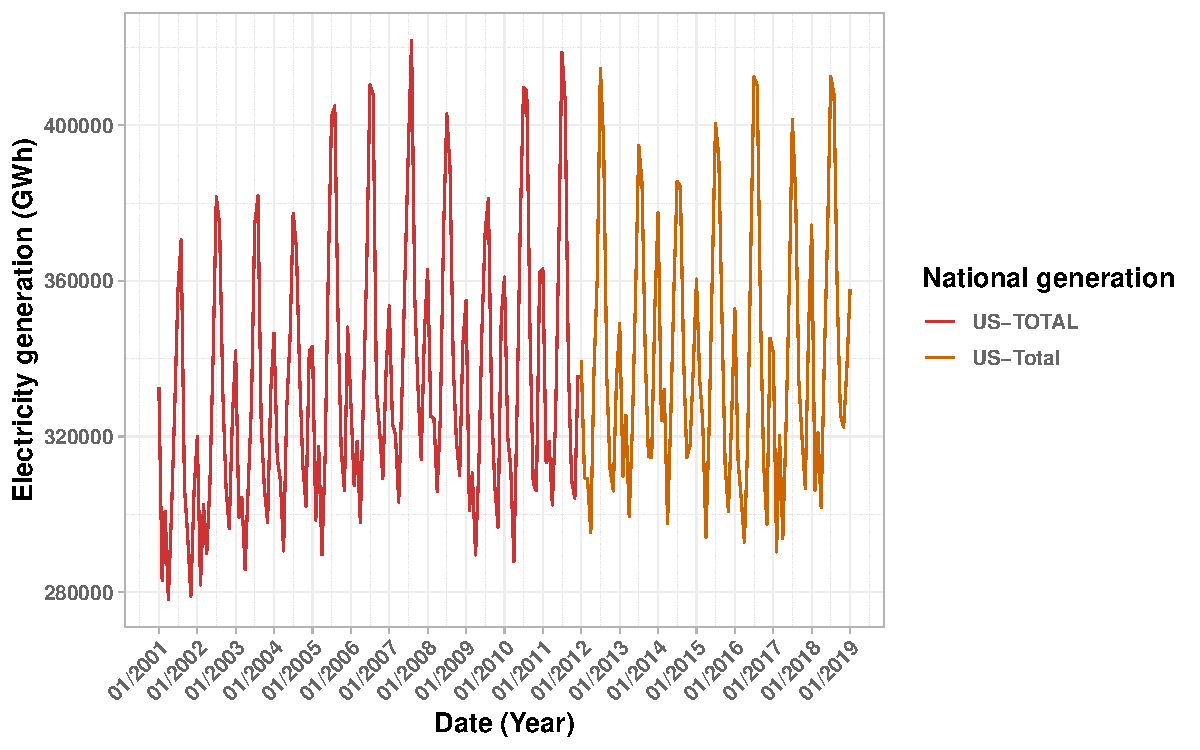
\includegraphics{Kara_ENV872_Project_files/figure-latex/unnamed-chunk-9-1.pdf}
\caption{National electricity generation}
\end{figure}

\begin{quote}
There was a small variation between the total states electricity
generation and the US summation as shown in the Table 7. A dataset using
only the states data was therefore used for the state level analysis and
a dataset including summation of generation across states was used for
the national level analysis. Date at the US-TOTAL and US-Total factor
level were therefore not used because of the slight discrepacy with
aggregated state values.
\end{quote}

\textbf{Plot of variation in electricity generation at the State level}

\begin{figure}
\centering
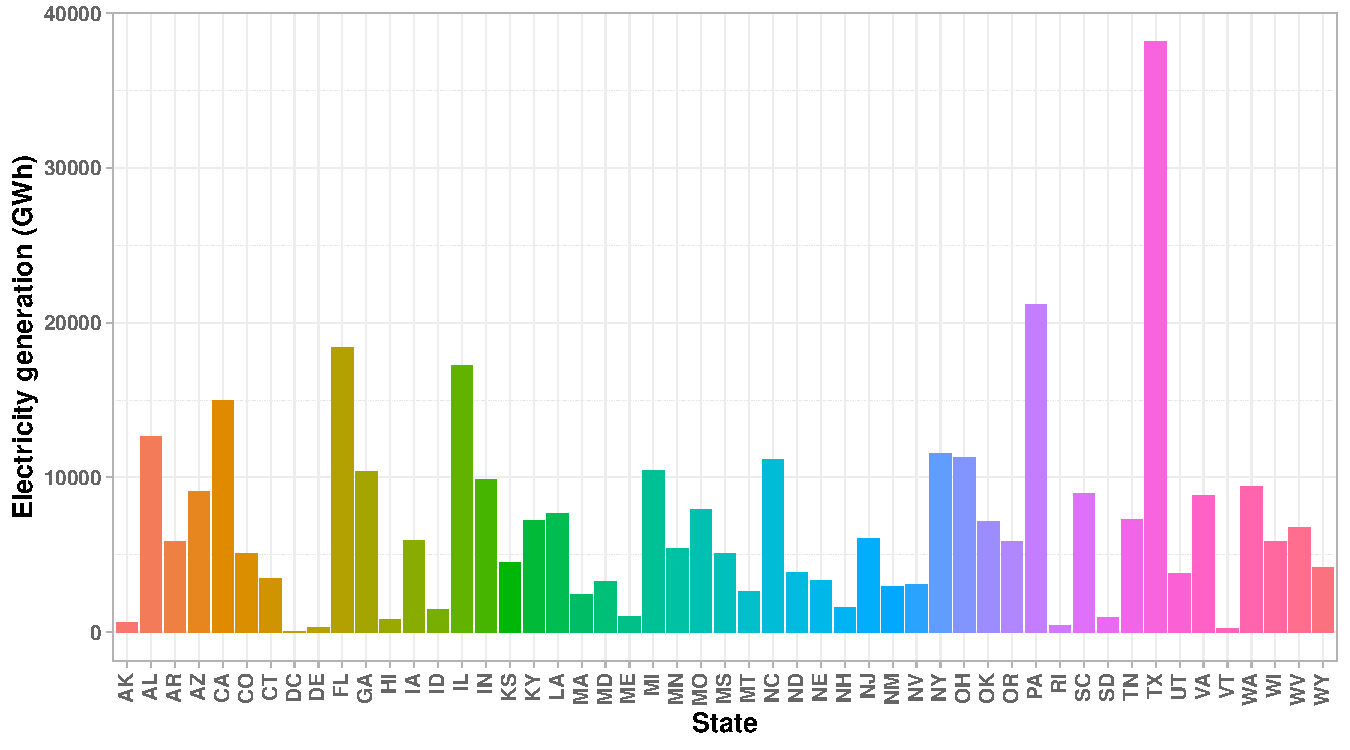
\includegraphics{Kara_ENV872_Project_files/figure-latex/unnamed-chunk-11-1.pdf}
\caption{Total electricity generation in Jan 2019 per state}
\end{figure}

\subsection{Data wrangling to create the main datasets for national and
state
level}\label{data-wrangling-to-create-the-main-datasets-for-national-and-state-level}

\subsubsection{Creation of first dataset -
EIA.data.by\_state}\label{creation-of-first-dataset---eia.data.by_state}

\begin{quote}
To obtain the first dataset for data analysis, EIA.data.by\_state, the
EIA.data.2001\_2019 raw dataset was wrangled as shown in the code below
to include only the Total Electric Power Industry which is a summation
of all producer codes as shown in the Table 6 and to remove US national
totals. The data wrangling was also done to spread data according to MWh
generation of each energy source and to combine the year and month
collumn into one date variable. The final dataset, EIA.data.by\_state,
includes the following variables of interest: Date, State, Geothermal,
Hydro,Other.Biomass, Solar, Wind, Wood.products, Renewable.total, Coal,
Nat.Gas, Petroleum, Total
\end{quote}

\begin{Shaded}
\begin{Highlighting}[]
\NormalTok{EIA.data.by_state <-}\StringTok{ }\NormalTok{EIA.data.2001_}\DecValTok{2019} \OperatorTok
\StringTok{  }\KeywordTok{filter}\NormalTok{(TYPE.OF.PRODUCER}\OperatorTok{==}\StringTok{"Total Electric Power Industry"}\NormalTok{) }\OperatorTok
\StringTok{  }\KeywordTok{filter}\NormalTok{(STATE}\OperatorTok{!=}\StringTok{ "US-TOTAL"} \OperatorTok{&}\StringTok{ }\NormalTok{STATE}\OperatorTok{!=}\StringTok{ "US-Total"}\NormalTok{) }\OperatorTok
\StringTok{  }\KeywordTok{spread}\NormalTok{(ENERGY.SOURCE,GENERATION..Megawatthours.) }\OperatorTok
\StringTok{  }\KeywordTok{mutate}\NormalTok{(}\DataTypeTok{Geothermal =}\KeywordTok{ifelse}\NormalTok{(}\KeywordTok{is.na}\NormalTok{(Geothermal),}\DecValTok{0}\NormalTok{,Geothermal)) }\OperatorTok
\StringTok{  }\KeywordTok{mutate}\NormalTok{(}\DataTypeTok{Hydro =} \KeywordTok{ifelse}\NormalTok{(}\KeywordTok{is.na}\NormalTok{(}\StringTok{`}\DataTypeTok{Hydroelectric Conventional}\StringTok{`}\NormalTok{),}
                        \DecValTok{0}\NormalTok{,}\StringTok{`}\DataTypeTok{Hydroelectric Conventional}\StringTok{`}\NormalTok{)) }\OperatorTok
\StringTok{  }\KeywordTok{mutate}\NormalTok{(}\DataTypeTok{Other.Biomass =} \KeywordTok{ifelse}\NormalTok{(}\KeywordTok{is.na}\NormalTok{(}\StringTok{`}\DataTypeTok{Other Biomass}\StringTok{`}\NormalTok{),}
                                \DecValTok{0}\NormalTok{,}\StringTok{`}\DataTypeTok{Other Biomass}\StringTok{`}\NormalTok{)) }\OperatorTok
\StringTok{  }\KeywordTok{mutate}\NormalTok{(}\DataTypeTok{Solar =} \KeywordTok{ifelse}\NormalTok{(}\KeywordTok{is.na}\NormalTok{(}\StringTok{`}\DataTypeTok{Solar Thermal and Photovoltaic}\StringTok{`}\NormalTok{),}
                        \DecValTok{0}\NormalTok{,}\StringTok{`}\DataTypeTok{Solar Thermal and Photovoltaic}\StringTok{`}\NormalTok{)) }\OperatorTok
\StringTok{  }\KeywordTok{mutate}\NormalTok{(}\DataTypeTok{Wind =} \KeywordTok{ifelse}\NormalTok{(}\KeywordTok{is.na}\NormalTok{(Wind),}\DecValTok{0}\NormalTok{,Wind)) }\OperatorTok
\StringTok{  }\KeywordTok{mutate}\NormalTok{(}\DataTypeTok{Wood.products =} \KeywordTok{ifelse}\NormalTok{(}\KeywordTok{is.na}\NormalTok{(}\StringTok{`}\DataTypeTok{Wood and Wood Derived Fuels}\StringTok{`}\NormalTok{),}
                                \DecValTok{0}\NormalTok{,}\StringTok{`}\DataTypeTok{Wood and Wood Derived Fuels}\StringTok{`}\NormalTok{)) }\OperatorTok
\StringTok{  }\KeywordTok{mutate}\NormalTok{(}\DataTypeTok{Renewable.total =}\NormalTok{ Geothermal}\OperatorTok{+}\NormalTok{Hydro}\OperatorTok{+}\NormalTok{Other.Biomass}\OperatorTok{+}
\StringTok{           }\NormalTok{Solar}\OperatorTok{+}\NormalTok{Wind}\OperatorTok{+}\NormalTok{Wood.products) }\OperatorTok
\StringTok{  }\KeywordTok{mutate}\NormalTok{(}\DataTypeTok{Coal =} \KeywordTok{ifelse}\NormalTok{(}\KeywordTok{is.na}\NormalTok{(Coal),}\DecValTok{0}\NormalTok{,Coal)) }\OperatorTok
\StringTok{  }\KeywordTok{mutate}\NormalTok{(}\DataTypeTok{Nat.Gas =} \KeywordTok{ifelse}\NormalTok{(}\KeywordTok{is.na}\NormalTok{(}\StringTok{`}\DataTypeTok{Natural Gas}\StringTok{`}\NormalTok{),}
                          \DecValTok{0}\NormalTok{,}\StringTok{`}\DataTypeTok{Natural Gas}\StringTok{`}\NormalTok{)) }\OperatorTok
\StringTok{  }\KeywordTok{mutate}\NormalTok{(}\DataTypeTok{Petroleum =} \KeywordTok{ifelse}\NormalTok{(}\KeywordTok{is.na}\NormalTok{(Petroleum),}
                            \DecValTok{0}\NormalTok{,Petroleum)) }\OperatorTok
\StringTok{  }\KeywordTok{mutate}\NormalTok{(}\DataTypeTok{Nuclear =} \KeywordTok{ifelse}\NormalTok{(}\KeywordTok{is.na}\NormalTok{(Nuclear),}
                          \DecValTok{0}\NormalTok{,Nuclear)) }\OperatorTok
\StringTok{  }\KeywordTok{mutate}\NormalTok{(}\DataTypeTok{Date =} \KeywordTok{make_date}\NormalTok{(YEAR,MONTH)) }\OperatorTok
\StringTok{  }\KeywordTok{select}\NormalTok{(Date, STATE, Geothermal,Hydro,}
\NormalTok{         Other.Biomass,Solar,Wind, Wood.products,}
\NormalTok{         Coal,Nat.Gas,Petroleum,}
\NormalTok{         Nuclear,Renewable.total,Total)}
\end{Highlighting}
\end{Shaded}

\subsubsection{Creation of second dataset -
EIA.data.national}\label{creation-of-second-dataset---eia.data.national}

\begin{quote}
A second analysis dataset was created to represent national electricity
generation across various energy sources by summing state level values
as shown in the wrangling code below.
\end{quote}

\begin{Shaded}
\begin{Highlighting}[]
\NormalTok{EIA.data.national <-}\StringTok{ }\NormalTok{EIA.data.by_state }\OperatorTok
\StringTok{  }\KeywordTok{group_by}\NormalTok{(Date) }\OperatorTok
\StringTok{  }\KeywordTok{summarise}\NormalTok{(}\DataTypeTok{National.Geothermal =} \KeywordTok{sum}\NormalTok{(Geothermal),}
            \DataTypeTok{National.Hydro =} \KeywordTok{sum}\NormalTok{(Hydro),}
            \DataTypeTok{National.Other.Biomass =} \KeywordTok{sum}\NormalTok{(Other.Biomass),}
            \DataTypeTok{National.Solar =} \KeywordTok{sum}\NormalTok{(Solar),}
            \DataTypeTok{National.Wind =} \KeywordTok{sum}\NormalTok{(Wind),}
            \DataTypeTok{National.wood.products =} \KeywordTok{sum}\NormalTok{(Wood.products),}
            \DataTypeTok{National.Coal =} \KeywordTok{sum}\NormalTok{(Coal),}
            \DataTypeTok{National.Nat.Gas =} \KeywordTok{sum}\NormalTok{(Nat.Gas),}
            \DataTypeTok{National.Petroleum =} \KeywordTok{sum}\NormalTok{(Petroleum),}
            \DataTypeTok{National.Nuclear =}\KeywordTok{sum}\NormalTok{(Nuclear),}
            \DataTypeTok{National.Renewable.total =} \KeywordTok{sum}\NormalTok{(Renewable.total),}
            \DataTypeTok{National.Total =} \KeywordTok{sum}\NormalTok{(Total))}
\end{Highlighting}
\end{Shaded}

\subsubsection{Data exploration of created
datasets}\label{data-exploration-of-created-datasets}

\begin{quote}
Table 8 shows the summary statistics for the electricity generation from
all the selected energy sources including total renewable energy
(Renewable.total variable) and all the energy sources (Total variable).
\end{quote}

\begin{table}

\caption{\label{tab:unnamed-chunk-14}Summary statistics for electricity generation (MWh) by energy source for all states}
\centering
\resizebox{\linewidth}{!}{
\begin{tabular}[t]{l|r|r|r|r|r|r|r|r}
\hline
  & N.Valid & Pct.Valid & Mean & Std.Dev & Min & Median & Max & IQR\\
\hline
Geothermal & 11067 & 100 & 25052.51 & 147441.44 & -140 & 0 & 1147970 & 0.0\\
\hline
Hydro & 11067 & 100 & 440516.99 & 1076092.36 & 0 & 113029 & 11210102 & 250229.5\\
\hline
Other.Biomass & 11067 & 100 & 30067.67 & 47596.23 & -535 & 8299 & 265105 & 35747.0\\
\hline
Solar & 11067 & 100 & 20349.35 & 134828.70 & -3 & 0 & 3144661 & 1057.0\\
\hline
Wind & 11067 & 100 & 174190.36 & 494949.85 & 0 & 7651 & 7548279 & 135000.0\\
\hline
Wood.products & 11067 & 100 & 63761.44 & 89673.07 & -390 & 19501 & 685925 & 102163.5\\
\hline
Coal & 11067 & 100 & 2788475.91 & 2906988.91 & -5559 & 2157406 & 15815851 & 3475819.5\\
\hline
Nat.Gas & 11067 & 100 & 1627877.87 & 3063518.75 & -903 & 568015 & 28568297 & 1555542.0\\
\hline
Petroleum & 11067 & 100 & 94456.31 & 310868.65 & -3417 & 11224 & 5317378 & 55609.5\\
\hline
Nuclear & 11067 & 100 & 1294177.77 & 1719842.22 & -25629 & 798993 & 8871262 & 2213163.5\\
\hline
Renewable.total & 11067 & 100 & 753938.32 & 1349140.89 & 0 & 328044 & 11691617 & 547045.0\\
\hline
Total & 11067 & 100 & 6590294.65 & 6253557.87 & -1094 & 4738322 & 49047812 & 6287579.5\\
\hline
\end{tabular}}
\end{table}

\subsubsection{Data visualization of created
datasets}\label{data-visualization-of-created-datasets}

\textbf{Plot of national level electricity generation by main energy
sources across time}

\begin{figure}
\centering
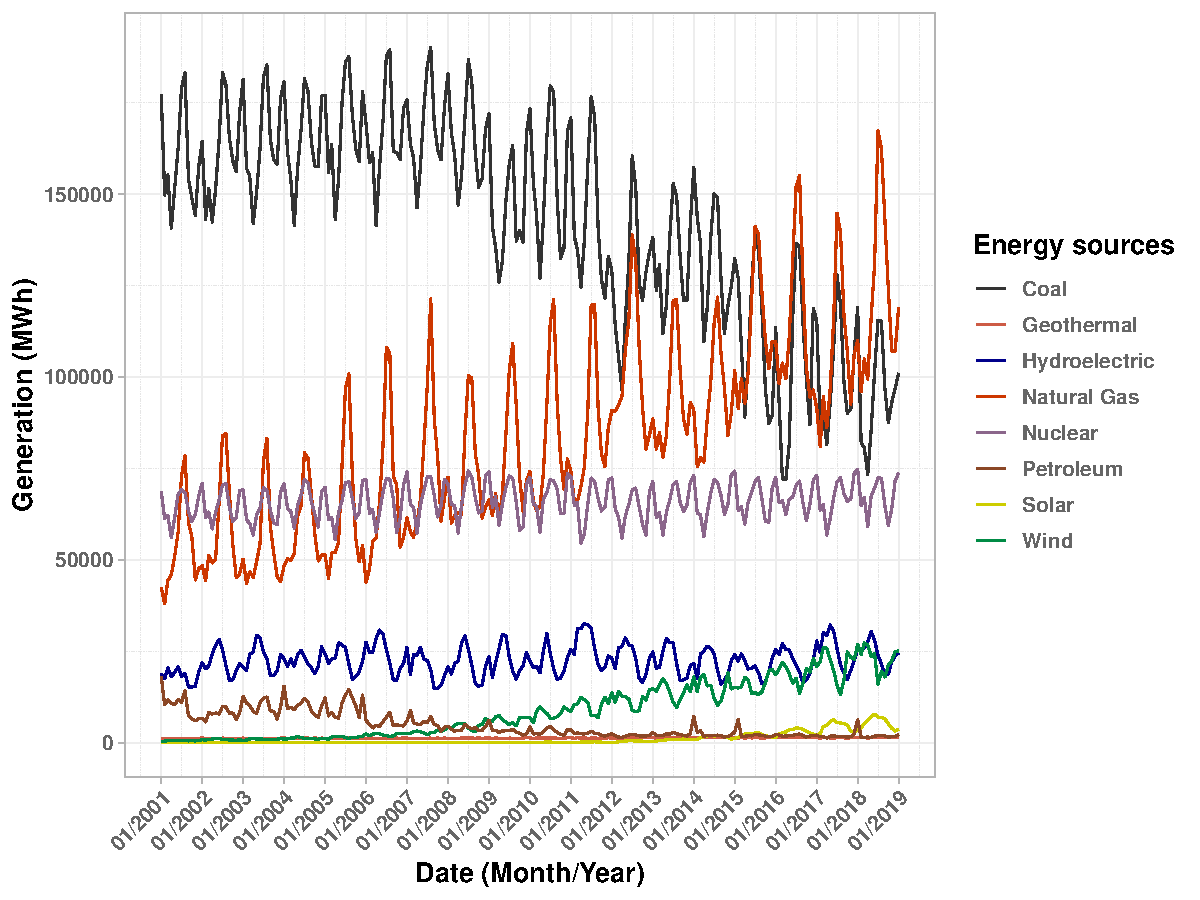
\includegraphics{Kara_ENV872_Project_files/figure-latex/unnamed-chunk-16-1.pdf}
\caption{National electricity generation by energy source}
\end{figure}

\newpage

\section{Analysis}\label{analysis}

\subsection{National level trend
analysis}\label{national-level-trend-analysis}

\subsubsection{Visualization of trends of major renewable and
non-renewable energy
sources}\label{visualization-of-trends-of-major-renewable-and-non-renewable-energy-sources}

\begin{quote}
Based on the data exploration and specifically figure 3, The major
renewable energy sources appear to be Hydroelectric power, wind energy
and solar energy. The major non renewable energy sources are coal
energy, natural gas energy and nuclear energy.
\end{quote}

\begin{figure}
\centering
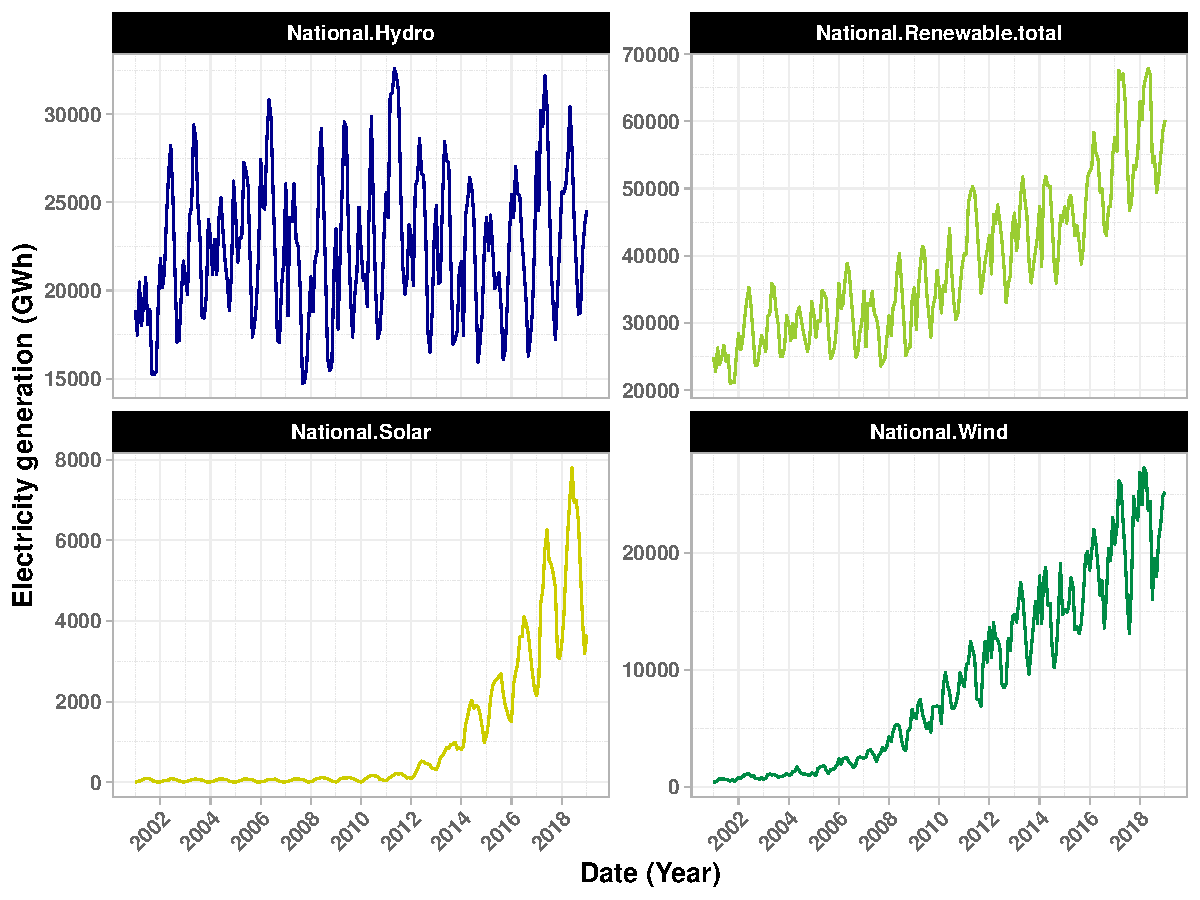
\includegraphics{Kara_ENV872_Project_files/figure-latex/unnamed-chunk-18-1.pdf}
\caption{Electricity generation by major renewable sources}
\end{figure}

\begin{quote}
Based on the series of the major renewable energy sources, hydroelectric
energy does not appear to have any incleasing trend therefore it is
unlikely that it has contributed to the visibly increasing growth in
total renewable energy generation at the national level. Solar and wind
energy however appear to have a similar increasing trend. The trend
analysis at the national level was therefore carried out on the solar
and wind series as well as the total renewable energy series.
\end{quote}

\begin{figure}
\centering
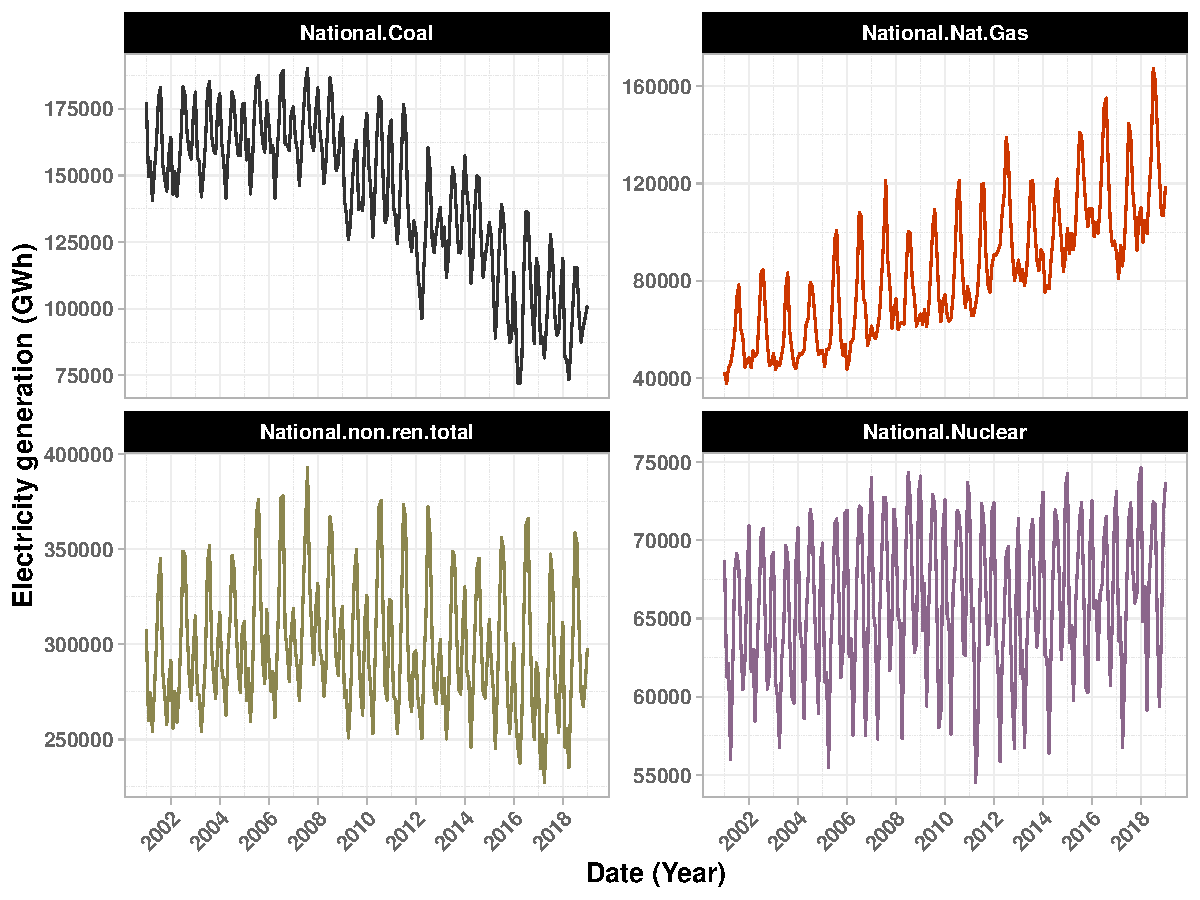
\includegraphics{Kara_ENV872_Project_files/figure-latex/unnamed-chunk-20-1.pdf}
\caption{Electricity generation by major renewable sources}
\end{figure}

\begin{quote}
Based on the series of the major non-renewable energy sources, nuclear
energy does not appear to have as significant a trend as coal and
Natural gas. It is therefore unlikely that it has contributed
significantly to the slight decrease in total non renewable energy
generation at the national level. The trend analysis at the national
level was therefore carried out on the coal and natural gas series.
\end{quote}

\subsubsection{Trend analysis of major renewable and non-renewable
energy
series.}\label{trend-analysis-of-major-renewable-and-non-renewable-energy-series.}

\paragraph{Changing to timeseries data and removing
seasonality}\label{changing-to-timeseries-data-and-removing-seasonality}

\begin{quote}
It was necessary to change the energy series into time series and to
remove the obvious seasonality so as to be able to carry out trend
analysis tests.
\end{quote}

\begin{Shaded}
\begin{Highlighting}[]
\CommentTok{#Changing series of interest into timeseries data}
\NormalTok{Nat.Solar.ts.data <-}\StringTok{ }\KeywordTok{ts}\NormalTok{(EIA.data.national[,}\DecValTok{5}\NormalTok{], }
                        \DataTypeTok{start =} \KeywordTok{c}\NormalTok{(}\DecValTok{2001}\NormalTok{,}\DecValTok{01}\NormalTok{), }\DataTypeTok{end=}\KeywordTok{c}\NormalTok{(}\DecValTok{2019}\NormalTok{,}\DecValTok{1}\NormalTok{),}\DataTypeTok{frequency =} \DecValTok{12}\NormalTok{)}
\NormalTok{Nat.Wind.ts.data <-}\StringTok{ }\KeywordTok{ts}\NormalTok{(EIA.data.national[,}\DecValTok{6}\NormalTok{], }
                       \DataTypeTok{start =} \KeywordTok{c}\NormalTok{(}\DecValTok{2001}\NormalTok{,}\DecValTok{01}\NormalTok{), }\DataTypeTok{end=}\KeywordTok{c}\NormalTok{(}\DecValTok{2019}\NormalTok{,}\DecValTok{1}\NormalTok{),}\DataTypeTok{frequency =} \DecValTok{12}\NormalTok{)}
\NormalTok{Nat.Renewable.ts.data <-}\StringTok{ }\KeywordTok{ts}\NormalTok{(EIA.data.national[,}\DecValTok{12}\NormalTok{], }
                            \DataTypeTok{start =} \KeywordTok{c}\NormalTok{(}\DecValTok{2001}\NormalTok{,}\DecValTok{01}\NormalTok{), }\DataTypeTok{end=}\KeywordTok{c}\NormalTok{(}\DecValTok{2019}\NormalTok{,}\DecValTok{1}\NormalTok{),}\DataTypeTok{frequency =} \DecValTok{12}\NormalTok{)}
\NormalTok{Nat.Coal.ts.data <-}\StringTok{ }\KeywordTok{ts}\NormalTok{(EIA.data.national[,}\DecValTok{8}\NormalTok{], }
                       \DataTypeTok{start =} \KeywordTok{c}\NormalTok{(}\DecValTok{2001}\NormalTok{,}\DecValTok{01}\NormalTok{), }\DataTypeTok{end=}\KeywordTok{c}\NormalTok{(}\DecValTok{2019}\NormalTok{,}\DecValTok{1}\NormalTok{),}\DataTypeTok{frequency =} \DecValTok{12}\NormalTok{)}
\NormalTok{Nat.Gas.ts.data <-}\StringTok{ }\KeywordTok{ts}\NormalTok{(EIA.data.national[,}\DecValTok{9}\NormalTok{], }
                      \DataTypeTok{start =} \KeywordTok{c}\NormalTok{(}\DecValTok{2001}\NormalTok{,}\DecValTok{01}\NormalTok{), }\DataTypeTok{end=}\KeywordTok{c}\NormalTok{(}\DecValTok{2019}\NormalTok{,}\DecValTok{1}\NormalTok{),}\DataTypeTok{frequency =} \DecValTok{12}\NormalTok{)}

\NormalTok{##Removing seasonality}
\NormalTok{##Removing seasonality in solar series}
\NormalTok{Nat.Solar.decomp <-}\StringTok{ }\KeywordTok{decompose}\NormalTok{(Nat.Solar.ts.data)}
\NormalTok{deseasonal_Nat.Solar <-}\StringTok{ }\KeywordTok{seasadj}\NormalTok{(Nat.Solar.decomp)}

\NormalTok{##Removing seasonality in wind series}
\NormalTok{Nat.Wind.decomp <-}\StringTok{ }\KeywordTok{decompose}\NormalTok{(Nat.Wind.ts.data)}
\NormalTok{deseasonal_Nat.Wind <-}\StringTok{ }\KeywordTok{seasadj}\NormalTok{(Nat.Wind.decomp)}

\NormalTok{##Removing seasonality in renewable series}
\NormalTok{Nat.Renewable.decomp <-}\StringTok{ }\KeywordTok{decompose}\NormalTok{(Nat.Renewable.ts.data)}
\NormalTok{deseasonal_Nat.Renewable <-}\StringTok{ }\KeywordTok{seasadj}\NormalTok{(Nat.Renewable.decomp)}

\NormalTok{##Removing seasonality in coal series}
\NormalTok{Nat.Coal.decomp <-}\StringTok{ }\KeywordTok{decompose}\NormalTok{(Nat.Coal.ts.data)}
\NormalTok{deseasonal_Nat.Coal <-}\StringTok{ }\KeywordTok{seasadj}\NormalTok{(Nat.Coal.decomp)}

\NormalTok{##Removing seasonality in natural gas series}
\NormalTok{Nat.Gas.decomp <-}\StringTok{ }\KeywordTok{decompose}\NormalTok{(Nat.Gas.ts.data)}
\NormalTok{deseasonal_Nat.Gas <-}\StringTok{ }\KeywordTok{seasadj}\NormalTok{(Nat.Gas.decomp)}
\end{Highlighting}
\end{Shaded}

\paragraph{Carrying out ADF and Mankandal trend
test}\label{carrying-out-adf-and-mankandal-trend-test}

\subparagraph{ADF trend tests on
series}\label{adf-trend-tests-on-series}

\begin{quote}
To test for a stochastic trend in the series, and ADF trend test was
carried out
\end{quote}

\begin{Shaded}
\begin{Highlighting}[]
\CommentTok{#Checking for a stochastic trend with ADF test on solar series }
\KeywordTok{adf.test}\NormalTok{(deseasonal_Nat.Solar, }\DataTypeTok{alternative =} \StringTok{"stationary"}\NormalTok{)}
\end{Highlighting}
\end{Shaded}

\begin{verbatim}
## 
##  Augmented Dickey-Fuller Test
## 
## data:  deseasonal_Nat.Solar
## Dickey-Fuller = -0.90921, Lag order = 5, p-value = 0.9506
## alternative hypothesis: stationary
\end{verbatim}

\begin{Shaded}
\begin{Highlighting}[]
\CommentTok{#Checking for a stochastic trend with ADF test on wind series }
\KeywordTok{adf.test}\NormalTok{(deseasonal_Nat.Wind, }\DataTypeTok{alternative =} \StringTok{"stationary"}\NormalTok{)}
\end{Highlighting}
\end{Shaded}

\begin{verbatim}
## 
##  Augmented Dickey-Fuller Test
## 
## data:  deseasonal_Nat.Wind
## Dickey-Fuller = -3.2801, Lag order = 5, p-value = 0.07573
## alternative hypothesis: stationary
\end{verbatim}

\begin{Shaded}
\begin{Highlighting}[]
\CommentTok{#Checking for a stochastic trend with ADF test on total renewable energy series }
\KeywordTok{adf.test}\NormalTok{(deseasonal_Nat.Renewable, }\DataTypeTok{alternative =} \StringTok{"stationary"}\NormalTok{)}
\end{Highlighting}
\end{Shaded}

\begin{verbatim}
## 
##  Augmented Dickey-Fuller Test
## 
## data:  deseasonal_Nat.Renewable
## Dickey-Fuller = -3.2402, Lag order = 5, p-value = 0.08238
## alternative hypothesis: stationary
\end{verbatim}

\begin{Shaded}
\begin{Highlighting}[]
\CommentTok{#Checking for a stochastic trend with ADF test on coal series }
\KeywordTok{adf.test}\NormalTok{(deseasonal_Nat.Coal, }\DataTypeTok{alternative =} \StringTok{"stationary"}\NormalTok{)}
\end{Highlighting}
\end{Shaded}

\begin{verbatim}
## 
##  Augmented Dickey-Fuller Test
## 
## data:  deseasonal_Nat.Coal
## Dickey-Fuller = -2.6226, Lag order = 5, p-value = 0.3148
## alternative hypothesis: stationary
\end{verbatim}

\begin{Shaded}
\begin{Highlighting}[]
\CommentTok{#Checking for a stochastic trend with ADF test on natural gas series }
\KeywordTok{adf.test}\NormalTok{(deseasonal_Nat.Gas, }\DataTypeTok{alternative =} \StringTok{"stationary"}\NormalTok{)}
\end{Highlighting}
\end{Shaded}

\begin{verbatim}
## 
##  Augmented Dickey-Fuller Test
## 
## data:  deseasonal_Nat.Gas
## Dickey-Fuller = -3.9301, Lag order = 5, p-value = 0.01354
## alternative hypothesis: stationary
\end{verbatim}

\begin{quote}
The null hypothesis of the ADF test is that a stochastic trend is
present in the series. The test results indicate that the following
series have a stochastic trend.
\end{quote}

\begin{itemize}
\tightlist
\item
  The national solar energy series (p-value = 0.9506)
\item
  The national wind energy series (p-value = 0.07573)
\item
  The national total renewable energy series (p-value = 0.08238)
\item
  The national coal energy series (p-value = 0.3148)
\end{itemize}

\begin{quote}
The national natural gas series has a low p value (p-value = 0.01354)
indicating it does not have a stochastic trend. A Man Kendall test to
test for a deterministic trend in the series was therefore carried out.
\end{quote}

\subparagraph{Mann-Kendall trend tests on natural gas
series}\label{mann-kendall-trend-tests-on-natural-gas-series}

\begin{Shaded}
\begin{Highlighting}[]
\CommentTok{#Checking for a monotonic trend using the Mann Kendall Test}
\KeywordTok{MannKendall}\NormalTok{(deseasonal_Nat.Gas)}
\end{Highlighting}
\end{Shaded}

\begin{verbatim}
## tau = 0.817, 2-sided pvalue =< 2.22e-16
\end{verbatim}

\begin{quote}
The null hypothesis of the Mann-Kendall test is that there is no
monotonic trend. The low p value of the test (pvalue =\textless{}
2.22e-16) indicates that we should reject the null hypothesis for the
alternative that a monotonic trend is present in the natural gas series.
The trend is increasing (tau = 0.817)
\end{quote}

\subsubsection{Changepoint analysis of major renewable energy
sourcess.}\label{changepoint-analysis-of-major-renewable-energy-sourcess.}

\paragraph{Changepoint analysis for solar energy
series}\label{changepoint-analysis-for-solar-energy-series}

\begin{Shaded}
\begin{Highlighting}[]
\CommentTok{#analysis of first change point for solar series}
\KeywordTok{pettitt.test}\NormalTok{(deseasonal_Nat.Solar)}
\end{Highlighting}
\end{Shaded}

\begin{verbatim}
## 
##  Pettitt's test for single change-point detection
## 
## data:  deseasonal_Nat.Solar
## U* = 10750, p-value < 2.2e-16
## alternative hypothesis: two.sided
## sample estimates:
## probable change point at time K 
##                             130
\end{verbatim}

\begin{quote}
Low p-value (\textless{} 2.2e-16) indicates that there is a significant
changepoint at observation 130 which coresponds to the date 2011-10-01.
\end{quote}

\begin{Shaded}
\begin{Highlighting}[]
\CommentTok{#analysis of second change point for solar series}
\KeywordTok{pettitt.test}\NormalTok{(deseasonal_Nat.Solar[}\DecValTok{131}\OperatorTok{:}\DecValTok{217}\NormalTok{])}
\end{Highlighting}
\end{Shaded}

\begin{verbatim}
## 
##  Pettitt's test for single change-point detection
## 
## data:  deseasonal_Nat.Solar[131:217]
## U* = 1880, p-value = 2.978e-14
## alternative hypothesis: two.sided
## sample estimates:
## probable change point at time K 
##                              40
\end{verbatim}

\begin{quote}
Low p-value (2.978e-14) indicates that there is a significant
changepoint at observation 40 (170) which coresponds to the date
2015-02-01.
\end{quote}

\begin{Shaded}
\begin{Highlighting}[]
\CommentTok{#analysis of third change point for solar series}
\KeywordTok{pettitt.test}\NormalTok{(deseasonal_Nat.Solar[}\DecValTok{171}\OperatorTok{:}\DecValTok{217}\NormalTok{])}
\end{Highlighting}
\end{Shaded}

\begin{verbatim}
## 
##  Pettitt's test for single change-point detection
## 
## data:  deseasonal_Nat.Solar[171:217]
## U* = 532, p-value = 2.216e-07
## alternative hypothesis: two.sided
## sample estimates:
## probable change point at time K 
##                              24
\end{verbatim}

\begin{quote}
Low p-value (2.216e-07) indicates that there is a significant
changepoint at observation 24 (194) which coresponds to the date
2017-02-01.
\end{quote}

\begin{Shaded}
\begin{Highlighting}[]
\CommentTok{#analysis of fourth change point for solar series}
\KeywordTok{pettitt.test}\NormalTok{(deseasonal_Nat.Solar[}\DecValTok{195}\OperatorTok{:}\DecValTok{217}\NormalTok{])}
\end{Highlighting}
\end{Shaded}

\begin{verbatim}
## 
##  Pettitt's test for single change-point detection
## 
## data:  deseasonal_Nat.Solar[195:217]
## U* = 64, p-value = 0.2886
## alternative hypothesis: two.sided
## sample estimates:
## probable change point at time K                            <NA> 
##                              12                              13
\end{verbatim}

\begin{quote}
the high p-value (0.2886) of the test indicates that there no other
significant changepoint.
\end{quote}

\textbf{Plot of National solar changepoints}

\begin{figure}
\centering
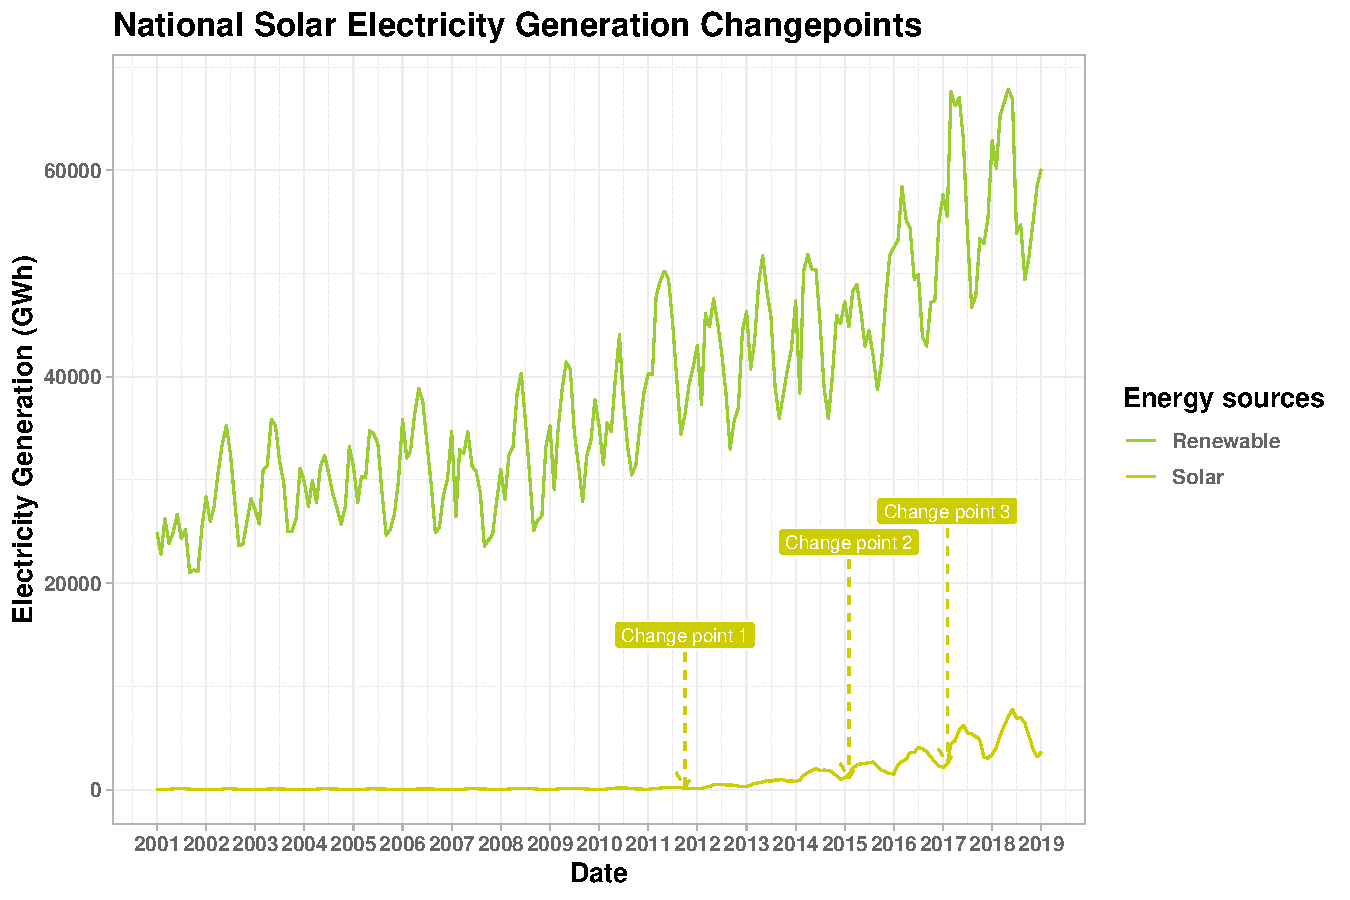
\includegraphics{Kara_ENV872_Project_files/figure-latex/unnamed-chunk-29-1.pdf}
\caption{National Solar Electricity Generation Changepoints}
\end{figure}

\paragraph{Changepoint analysis for wind energy
series}\label{changepoint-analysis-for-wind-energy-series}

\begin{Shaded}
\begin{Highlighting}[]
\CommentTok{#analysis of first change point for wind series}
\KeywordTok{pettitt.test}\NormalTok{(deseasonal_Nat.Wind)}
\end{Highlighting}
\end{Shaded}

\begin{verbatim}
## 
##  Pettitt's test for single change-point detection
## 
## data:  deseasonal_Nat.Wind
## U* = 11768, p-value < 2.2e-16
## alternative hypothesis: two.sided
## sample estimates:
## probable change point at time K 
##                             110
\end{verbatim}

\begin{quote}
Low p-value (\textless{} 2.2e-16) indicates that there is a significant
changepoint at observation 110 which coresponds to the date 2010-02-01.
\end{quote}

\begin{Shaded}
\begin{Highlighting}[]
\CommentTok{#analysis of second change point for wind series}
\KeywordTok{pettitt.test}\NormalTok{(deseasonal_Nat.Wind[}\DecValTok{111}\OperatorTok{:}\DecValTok{217}\NormalTok{])}
\end{Highlighting}
\end{Shaded}

\begin{verbatim}
## 
##  Pettitt's test for single change-point detection
## 
## data:  deseasonal_Nat.Wind[111:217]
## U* = 2672, p-value = 1.8e-15
## alternative hypothesis: two.sided
## sample estimates:
## probable change point at time K 
##                              56
\end{verbatim}

\begin{quote}
Low p-value (1.8e-15) indicates that there is a significant changepoint
at observation 56 (166) which coresponds to the date 2014-10-01.
\end{quote}

\begin{Shaded}
\begin{Highlighting}[]
\CommentTok{#analysis of third change point for wind series}
\KeywordTok{pettitt.test}\NormalTok{(deseasonal_Nat.Wind[}\DecValTok{167}\OperatorTok{:}\DecValTok{217}\NormalTok{])}
\end{Highlighting}
\end{Shaded}

\begin{verbatim}
## 
##  Pettitt's test for single change-point detection
## 
## data:  deseasonal_Nat.Wind[167:217]
## U* = 542, p-value = 4.379e-06
## alternative hypothesis: two.sided
## sample estimates:
## probable change point at time K 
##                              23
\end{verbatim}

\begin{quote}
Low p-value (4.379e-06) indicates that there is a significant
changepoint at observation 23 (189) which coresponds to the date
2016-09-01.
\end{quote}

\begin{Shaded}
\begin{Highlighting}[]
\CommentTok{#analysis of fourth change point for solar series}
\KeywordTok{pettitt.test}\NormalTok{(deseasonal_Nat.Wind[}\DecValTok{190}\OperatorTok{:}\DecValTok{217}\NormalTok{])}
\end{Highlighting}
\end{Shaded}

\begin{verbatim}
## 
##  Pettitt's test for single change-point detection
## 
## data:  deseasonal_Nat.Wind[190:217]
## U* = 108, p-value = 0.09209
## alternative hypothesis: two.sided
## sample estimates:
## probable change point at time K 
##                              12
\end{verbatim}

\begin{quote}
the high p-value (0.09209) of the test indicates that there no other
significant changepoint.
\end{quote}

\textbf{Plot of National wind changepoints}

\begin{figure}
\centering
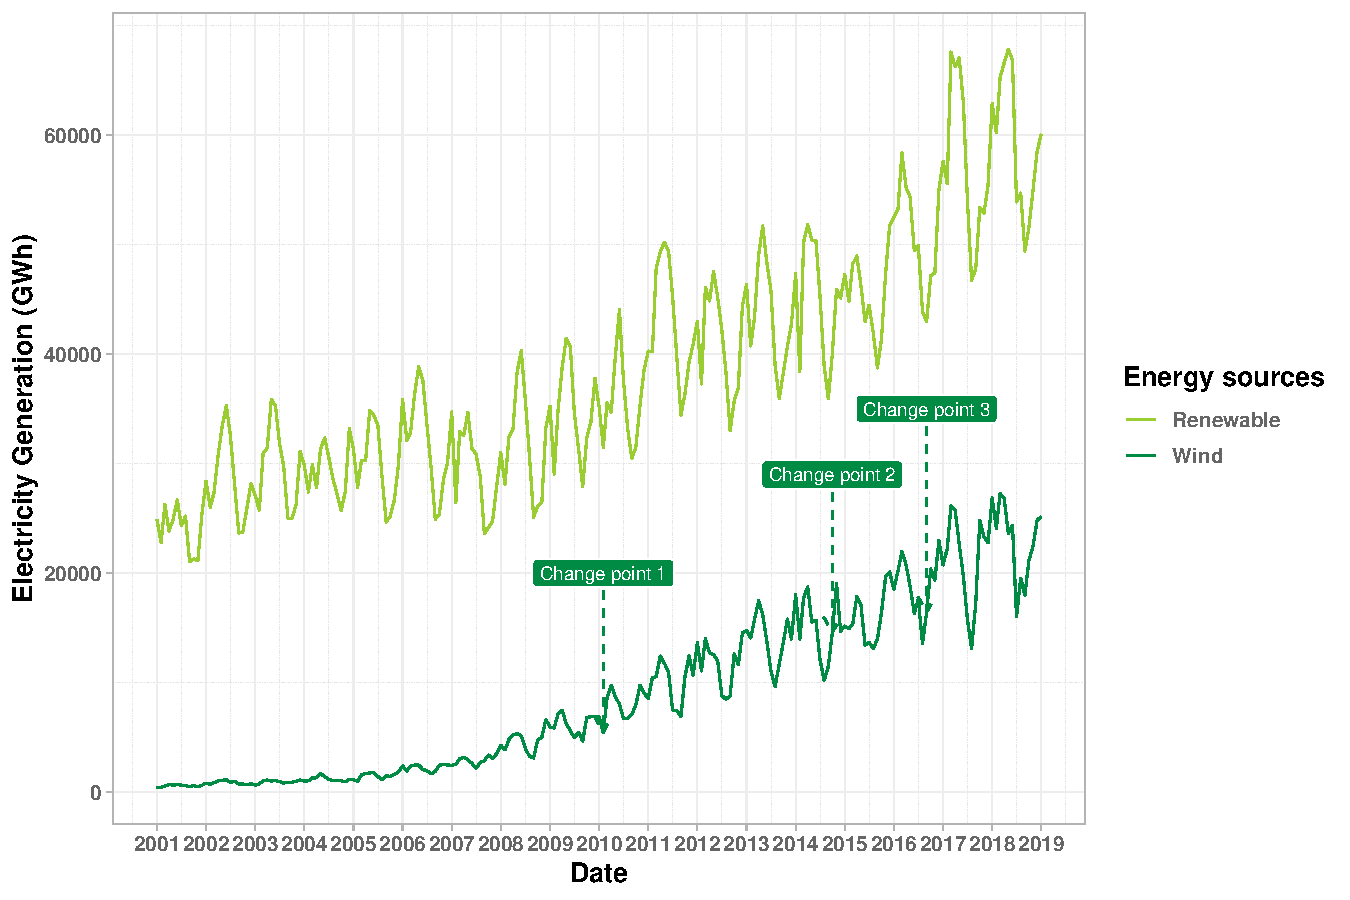
\includegraphics{Kara_ENV872_Project_files/figure-latex/unnamed-chunk-35-1.pdf}
\caption{National Wind Electricity Generation Changepoints}
\end{figure}

\subsection{State level trend
analysis}\label{state-level-trend-analysis}

\subsubsection{Trend analysis of wind energy in
Kansas.}\label{trend-analysis-of-wind-energy-in-kansas.}

\begin{quote}
A changepoint trend analysis was caried out for Kansas state to
determine whether renewable energy from wind follows a similar trend to
the national wind series
\end{quote}

\subparagraph{Kansas dataset}\label{kansas-dataset}

\begin{Shaded}
\begin{Highlighting}[]
\CommentTok{#Creating Kansas Dataset}
\NormalTok{data.KS.state <-}\StringTok{ }\NormalTok{EIA.data.by_state }\OperatorTok
\StringTok{  }\KeywordTok{filter}\NormalTok{(STATE}\OperatorTok{==}\StringTok{"KS"}\NormalTok{) }\OperatorTok
\StringTok{  }\KeywordTok{select}\NormalTok{(Date,Wind,Renewable.total,Total)}

\CommentTok{#Converting into time series}
\NormalTok{KS.Wind <-}\StringTok{ }\KeywordTok{ts}\NormalTok{(data.KS.state[,}\DecValTok{2}\NormalTok{], }\DataTypeTok{start =} \KeywordTok{c}\NormalTok{(}\DecValTok{2001}\NormalTok{,}\DecValTok{01}\NormalTok{), }
              \DataTypeTok{end=}\KeywordTok{c}\NormalTok{(}\DecValTok{2019}\NormalTok{,}\DecValTok{1}\NormalTok{),}\DataTypeTok{frequency =} \DecValTok{12}\NormalTok{)}
\NormalTok{KS.renewable <-}\StringTok{ }\KeywordTok{ts}\NormalTok{(data.KS.state[,}\DecValTok{3}\NormalTok{], }\DataTypeTok{start =} \KeywordTok{c}\NormalTok{(}\DecValTok{2001}\NormalTok{,}\DecValTok{01}\NormalTok{), }
                   \DataTypeTok{end=}\KeywordTok{c}\NormalTok{(}\DecValTok{2019}\NormalTok{,}\DecValTok{1}\NormalTok{),}\DataTypeTok{frequency =} \DecValTok{12}\NormalTok{)}
\NormalTok{KS.total <-}\StringTok{ }\KeywordTok{ts}\NormalTok{(data.KS.state[,}\DecValTok{4}\NormalTok{], }\DataTypeTok{start =} \KeywordTok{c}\NormalTok{(}\DecValTok{2001}\NormalTok{,}\DecValTok{01}\NormalTok{), }
               \DataTypeTok{end=}\KeywordTok{c}\NormalTok{(}\DecValTok{2019}\NormalTok{,}\DecValTok{1}\NormalTok{),}\DataTypeTok{frequency =} \DecValTok{12}\NormalTok{)}
\end{Highlighting}
\end{Shaded}

\paragraph{Removing seasonal component out in Kansas
series}\label{removing-seasonal-component-out-in-kansas-series}

\begin{Shaded}
\begin{Highlighting}[]
\CommentTok{#Removing seasonal component from wind series}
\NormalTok{KS.Wind.decomp <-}\StringTok{ }\KeywordTok{decompose}\NormalTok{(KS.Wind)}
\NormalTok{deseasonal_KS.Wind <-}\StringTok{ }\KeywordTok{seasadj}\NormalTok{(KS.Wind.decomp)}

\CommentTok{#Removing seasonal component from the renewable energy series}
\NormalTok{KS.renewable.decomp <-}\StringTok{ }\KeywordTok{decompose}\NormalTok{(KS.renewable)}
\NormalTok{deseasonal_KS.renewable <-}\StringTok{ }\KeywordTok{seasadj}\NormalTok{(KS.renewable.decomp)}

\CommentTok{#Checking for a stochastic trend with ADF test}
\KeywordTok{adf.test}\NormalTok{(deseasonal_KS.Wind, }\DataTypeTok{alternative =} \StringTok{"stationary"}\NormalTok{)}
\end{Highlighting}
\end{Shaded}

\begin{verbatim}
## 
##  Augmented Dickey-Fuller Test
## 
## data:  deseasonal_KS.Wind
## Dickey-Fuller = -1.5031, Lag order = 5, p-value = 0.7845
## alternative hypothesis: stationary
\end{verbatim}

\begin{Shaded}
\begin{Highlighting}[]
\KeywordTok{adf.test}\NormalTok{(deseasonal_KS.renewable, }\DataTypeTok{alternative =} \StringTok{"stationary"}\NormalTok{)}
\end{Highlighting}
\end{Shaded}

\begin{verbatim}
## 
##  Augmented Dickey-Fuller Test
## 
## data:  deseasonal_KS.renewable
## Dickey-Fuller = -1.5036, Lag order = 5, p-value = 0.7843
## alternative hypothesis: stationary
\end{verbatim}

\begin{quote}
The result of the ADF test of the Wind series (p=0.7845) indicates that
the series has a stochastic trend, this result is similar for the total
renewable energy series (p=0.7843).
\end{quote}

\paragraph{Changepoint analysis of wind energy
series}\label{changepoint-analysis-of-wind-energy-series}

\begin{Shaded}
\begin{Highlighting}[]
\CommentTok{#analysis of first change point}
\KeywordTok{pettitt.test}\NormalTok{(deseasonal_KS.Wind)}
\end{Highlighting}
\end{Shaded}

\begin{verbatim}
## 
##  Pettitt's test for single change-point detection
## 
## data:  deseasonal_KS.Wind
## U* = 11694, p-value < 2.2e-16
## alternative hypothesis: two.sided
## sample estimates:
## probable change point at time K 
##                             102
\end{verbatim}

\begin{quote}
small pvalues (\textless{} 2.2e-16) indicates a significant change point
was detected in both series in 2009-06-01 (102) for the wind series.
\end{quote}

\begin{Shaded}
\begin{Highlighting}[]
\CommentTok{#analysis of second change point}
\KeywordTok{pettitt.test}\NormalTok{(deseasonal_KS.Wind[}\DecValTok{103}\OperatorTok{:}\DecValTok{217}\NormalTok{])}
\end{Highlighting}
\end{Shaded}

\begin{verbatim}
## 
##  Pettitt's test for single change-point detection
## 
## data:  deseasonal_KS.Wind[103:217]
## U* = 3202, p-value < 2.2e-16
## alternative hypothesis: two.sided
## sample estimates:
## probable change point at time K 
##                              50
\end{verbatim}

\begin{quote}
small p value (\textless{} 2.2e-16) indicates a significant changepoint
at obs 50 (152). This changepoint occured at 2013-08-01.
\end{quote}

\begin{Shaded}
\begin{Highlighting}[]
\CommentTok{#analysis of third change point}
\KeywordTok{pettitt.test}\NormalTok{(deseasonal_KS.Wind[}\DecValTok{153}\OperatorTok{:}\DecValTok{217}\NormalTok{])}
\end{Highlighting}
\end{Shaded}

\begin{verbatim}
## 
##  Pettitt's test for single change-point detection
## 
## data:  deseasonal_KS.Wind[153:217]
## U* = 994, p-value = 1.17e-09
## alternative hypothesis: two.sided
## sample estimates:
## probable change point at time K 
##                              36
\end{verbatim}

\begin{quote}
small p value (1.17e-09) indicates a significant changepoint at obs 36
(188). This changepoint occured at 2016-08-01.
\end{quote}

\textbf{Plot of Kansas wind changepoints}

\begin{figure}
\centering
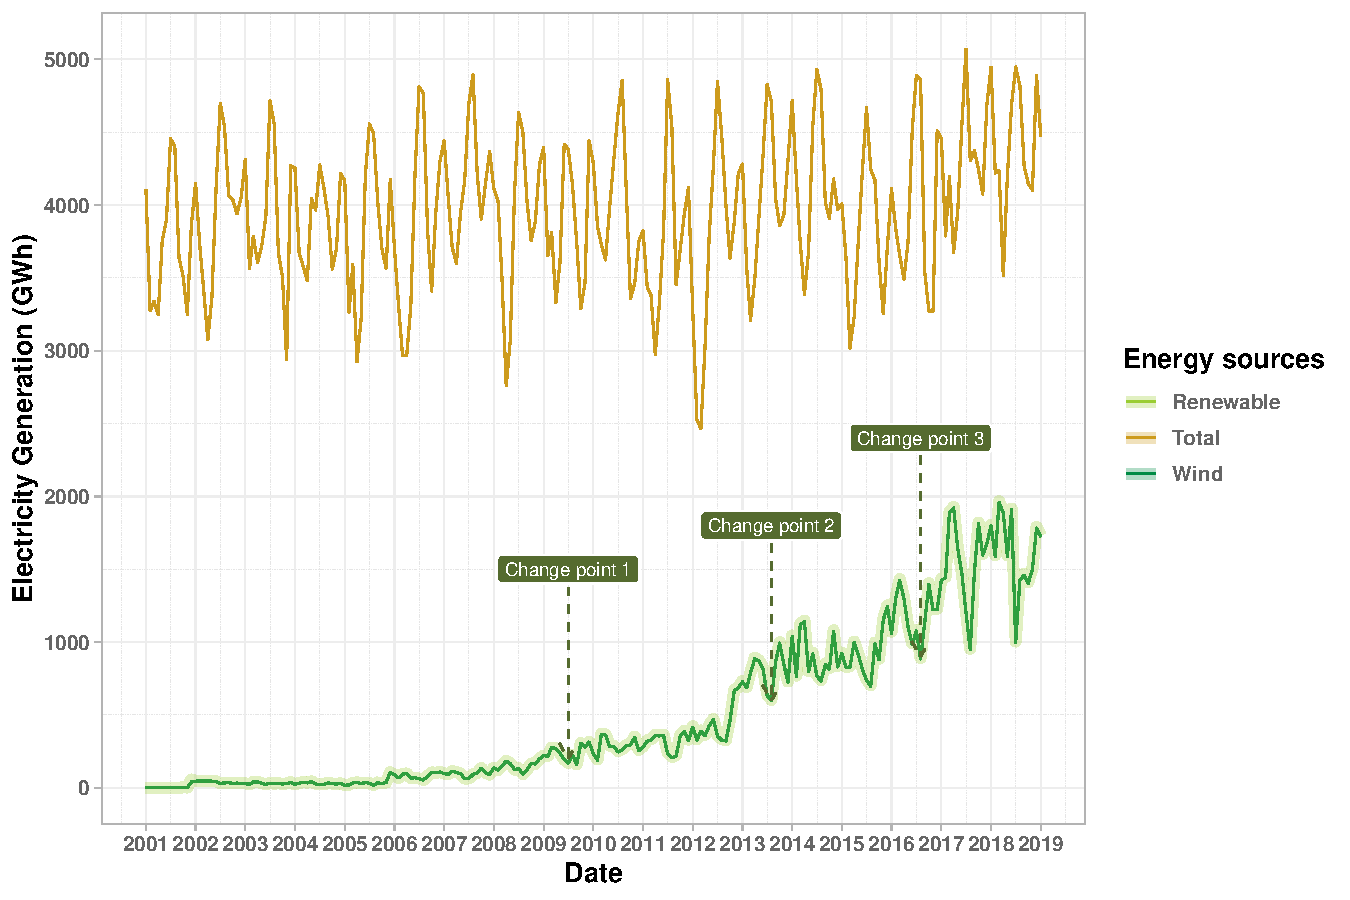
\includegraphics{Kara_ENV872_Project_files/figure-latex/unnamed-chunk-42-1.pdf}
\caption{Kansas wind electricity generation}
\end{figure}

\subsubsection{Trend analysis of solar energy in
California.}\label{trend-analysis-of-solar-energy-in-california.}

\subparagraph{California dataset}\label{california-dataset}

\begin{Shaded}
\begin{Highlighting}[]
\CommentTok{#Creating California Dataset}
\NormalTok{data.CA.state <-}\StringTok{ }\NormalTok{EIA.data.by_state }\OperatorTok
\StringTok{  }\KeywordTok{filter}\NormalTok{(STATE}\OperatorTok{==}\StringTok{"CA"}\NormalTok{) }\OperatorTok
\StringTok{  }\KeywordTok{select}\NormalTok{(Date,Solar,Renewable.total,Total)}

\CommentTok{#Converting into time series}
\NormalTok{CA.Solar <-}\StringTok{ }\KeywordTok{ts}\NormalTok{(data.CA.state[,}\DecValTok{2}\NormalTok{], }\DataTypeTok{start =} \KeywordTok{c}\NormalTok{(}\DecValTok{2001}\NormalTok{,}\DecValTok{01}\NormalTok{), }
               \DataTypeTok{end=}\KeywordTok{c}\NormalTok{(}\DecValTok{2019}\NormalTok{,}\DecValTok{1}\NormalTok{),}\DataTypeTok{frequency =} \DecValTok{12}\NormalTok{)}
\NormalTok{CA.renewable <-}\StringTok{ }\KeywordTok{ts}\NormalTok{(data.CA.state[,}\DecValTok{3}\NormalTok{], }\DataTypeTok{start =} \KeywordTok{c}\NormalTok{(}\DecValTok{2001}\NormalTok{,}\DecValTok{01}\NormalTok{), }
                   \DataTypeTok{end=}\KeywordTok{c}\NormalTok{(}\DecValTok{2019}\NormalTok{,}\DecValTok{1}\NormalTok{),}\DataTypeTok{frequency =} \DecValTok{12}\NormalTok{)}
\NormalTok{CA.total <-}\StringTok{ }\KeywordTok{ts}\NormalTok{(data.CA.state[,}\DecValTok{4}\NormalTok{], }\DataTypeTok{start =} \KeywordTok{c}\NormalTok{(}\DecValTok{2001}\NormalTok{,}\DecValTok{01}\NormalTok{), }
               \DataTypeTok{end=}\KeywordTok{c}\NormalTok{(}\DecValTok{2019}\NormalTok{,}\DecValTok{1}\NormalTok{),}\DataTypeTok{frequency =} \DecValTok{12}\NormalTok{)}
\end{Highlighting}
\end{Shaded}

\paragraph{Removing seasonal component out of California
series}\label{removing-seasonal-component-out-of-california-series}

\begin{Shaded}
\begin{Highlighting}[]
\CommentTok{#Removing seasonal component from solar series}
\NormalTok{CA.Solar.decomp <-}\StringTok{ }\KeywordTok{decompose}\NormalTok{(CA.Solar)}
\NormalTok{deseasonal_CA.Solar <-}\StringTok{ }\KeywordTok{seasadj}\NormalTok{(CA.Solar.decomp) }

\CommentTok{#Removing seasonal component from the renewable energy series}
\NormalTok{CA.renewable.decomp <-}\StringTok{ }\KeywordTok{decompose}\NormalTok{(CA.renewable)}
\NormalTok{deseasonal_CA.renewable <-}\StringTok{ }\KeywordTok{seasadj}\NormalTok{(CA.renewable.decomp) }

\CommentTok{#Checking for a stochastic trend with ADF test}
\KeywordTok{adf.test}\NormalTok{(deseasonal_CA.Solar, }\DataTypeTok{alternative =} \StringTok{"stationary"}\NormalTok{)}
\end{Highlighting}
\end{Shaded}

\begin{verbatim}
## 
##  Augmented Dickey-Fuller Test
## 
## data:  deseasonal_CA.Solar
## Dickey-Fuller = -1.6276, Lag order = 5, p-value = 0.7322
## alternative hypothesis: stationary
\end{verbatim}

\begin{Shaded}
\begin{Highlighting}[]
\KeywordTok{adf.test}\NormalTok{(deseasonal_CA.renewable, }\DataTypeTok{alternative =} \StringTok{"stationary"}\NormalTok{)}
\end{Highlighting}
\end{Shaded}

\begin{verbatim}
## 
##  Augmented Dickey-Fuller Test
## 
## data:  deseasonal_CA.renewable
## Dickey-Fuller = -2.7292, Lag order = 5, p-value = 0.2701
## alternative hypothesis: stationary
\end{verbatim}

\begin{quote}
The result of the ADF test of the solar series (p=0.7322) indicates that
the series has a stochastic trend. This result is similar for the total
renewable energy series (p=0.2701).
\end{quote}

\paragraph{Changepoint analysis of solar energy
series}\label{changepoint-analysis-of-solar-energy-series}

\begin{Shaded}
\begin{Highlighting}[]
\CommentTok{#analysis of first change point}
\KeywordTok{pettitt.test}\NormalTok{(deseasonal_CA.Solar)}
\end{Highlighting}
\end{Shaded}

\begin{verbatim}
## 
##  Pettitt's test for single change-point detection
## 
## data:  deseasonal_CA.Solar
## U* = 10398, p-value < 2.2e-16
## alternative hypothesis: two.sided
## sample estimates:
## probable change point at time K 
##                             142
\end{verbatim}

\begin{quote}
small p value (\textless{} 2.2e-16) indicates there a change point was
detected in the solar series in observation 142 corresponding to
2012-10-01.
\end{quote}

\begin{Shaded}
\begin{Highlighting}[]
\CommentTok{#analysis of second change point}
\KeywordTok{pettitt.test}\NormalTok{(deseasonal_CA.Solar[}\DecValTok{143}\OperatorTok{:}\DecValTok{217}\NormalTok{])}
\end{Highlighting}
\end{Shaded}

\begin{verbatim}
## 
##  Pettitt's test for single change-point detection
## 
## data:  deseasonal_CA.Solar[143:217]
## U* = 1342, p-value = 2.106e-11
## alternative hypothesis: two.sided
## sample estimates:
## probable change point at time K 
##                              39
\end{verbatim}

\begin{quote}
small p value (2.106e-11) indicates there a changepoint was detected at
observation 39 (181) corresponding to 2016-01-01.
\end{quote}

\begin{Shaded}
\begin{Highlighting}[]
\CommentTok{#analysis of third change point}
\KeywordTok{pettitt.test}\NormalTok{(deseasonal_CA.Solar[}\DecValTok{182}\OperatorTok{:}\DecValTok{217}\NormalTok{])}
\end{Highlighting}
\end{Shaded}

\begin{verbatim}
## 
##  Pettitt's test for single change-point detection
## 
## data:  deseasonal_CA.Solar[182:217]
## U* = 209, p-value = 0.00846
## alternative hypothesis: two.sided
## sample estimates:
## probable change point at time K 
##                              13
\end{verbatim}

\begin{quote}
small p value (0.00846)indicates there a changepoint was detected at
observation 13 (194) corresponding to 2017-02-01.
\end{quote}

\begin{Shaded}
\begin{Highlighting}[]
\CommentTok{#analysis of fourth change point}
\KeywordTok{pettitt.test}\NormalTok{(deseasonal_CA.Solar[}\DecValTok{195}\OperatorTok{:}\DecValTok{217}\NormalTok{])}
\end{Highlighting}
\end{Shaded}

\begin{verbatim}
## 
##  Pettitt's test for single change-point detection
## 
## data:  deseasonal_CA.Solar[195:217]
## U* = 50, p-value = 0.6137
## alternative hypothesis: two.sided
## sample estimates:
## probable change point at time K 
##                              13
\end{verbatim}

\begin{quote}
large p value (0.6137)indicates there is no other significant
changepoint.
\end{quote}

\textbf{Plot of California solar changepoints}

\begin{figure}
\centering
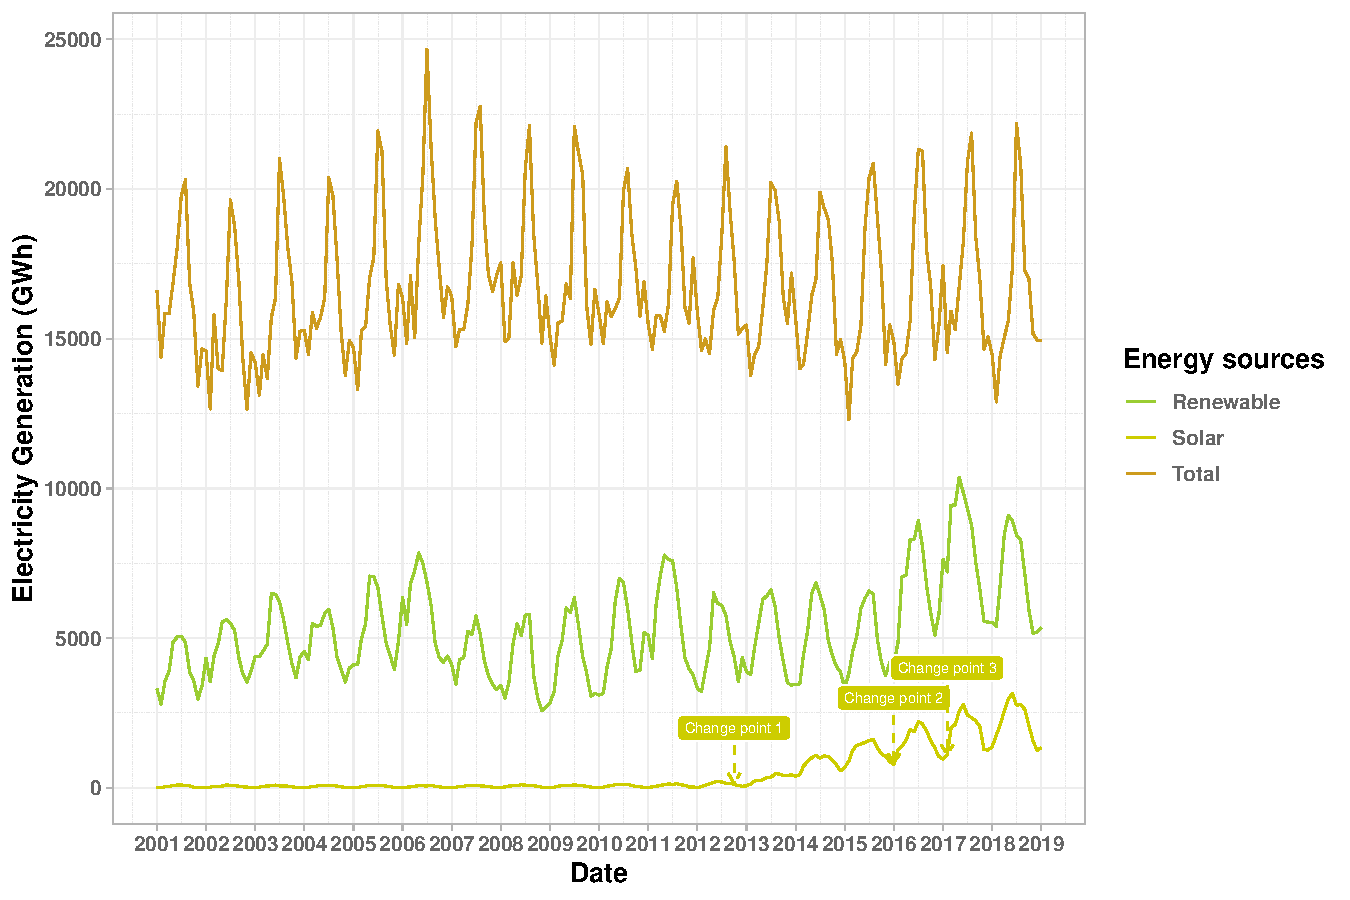
\includegraphics{Kara_ENV872_Project_files/figure-latex/unnamed-chunk-50-1.pdf}
\caption{California solar electricity generation}
\end{figure}

\newpage

\section{Summary and Conclusions}\label{summary-and-conclusions}

\begin{quote}
The table below summarizes the results of the changepoint analysis tests
for the electricity generation from solar energy at the national level
and in California and electricity generation from wind energy at the
national level and in Kansas.
\end{quote}

\begin{longtable}[]{@{}llll@{}}
\toprule
Dataset & Changepoint 1 & Changepoint 2 & Changepoint 3\tabularnewline
\midrule
\endhead
National solar energy & 10/2011 & 02/2015 & 02/2017\tabularnewline
National wind energy & 02/2010 & 10/2014 & 09/2016\tabularnewline
Kansas wind energy & 06/2009 & 08/2013 & 08/2016\tabularnewline
California solar energy & 10/2012 & 01/2016 & 02/2017\tabularnewline
\bottomrule
\end{longtable}

\begin{quote}
all analysed energy generation series had three changepoints. All
changepoints occur post 2008 indicating the rate of adoption of
renewable energy for electricity generation has changed in the last
decade, consistent with the literature. All changepoints indicate also
an increase in electricty generation from the renewable resource.
\end{quote}

\begin{quote}
Changepoint 1 and two at the national and state level do not appear to
be related for both wind energy and solar. Change point 3 for solar and
wind energy at the state and national level however coincide. This could
indicate that significant increase in renewable energy levels is being
driven by specific states and cannot neccessaritly be generalized to
all.
\end{quote}

\begin{quote}
The changepoint 1 in Kansas wind energy series coresponds to the year
the state adopted the RPS policy. Changepoint 2 does not correspond to
any policy change however it is the year Kansas reached its renewable
energy target of 20\% of its electricity generation being from renewable
resources. It was expected that a changepoint would be detected in 2015
or early 2016 due to the Kansa's decision to repeal its RPS policy and
change it from a mandatory goal to a voluntary one. A lack of clear
changepoint related to this indicates negative policy changes may not
have an immediate impact on adoption rates of renewable energy resource
as compared to positive ones.
\end{quote}

\begin{quote}
For California, changepoint 1 and 3 does not correspond to any major
renewable energy policy changes. A major policy revison however took
place in 2015 and could have resulted in a shift in the solar energy
trend as shown in changepoint 2.
\end{quote}

\begin{quote}
It is therefore probable that polciy changes have impacted the adoption
trends for wind and solar energy in Kansas and California, however more
analysis needs to be done in this area to be able to definitively
determine the causal relationship between policy changes and renewable
energy adoption.
\end{quote}


\end{document}
